% Document class
% Document class
% chktex-file 44
% chktex-file 13
% chktex-file 8
\documentclass[12pt,a4paper]{article}%

% Packages
\usepackage[utf8]{inputenc}%
\usepackage[T1]{fontenc}%
\usepackage{indentfirst}%
\usepackage{geometry}%
\usepackage{setspace}%
\usepackage{times}%
\usepackage{lipsum}% For dummy text
\usepackage{graphicx}%
\usepackage{fancyhdr}%
\usepackage{titlesec}%
\usepackage{tocloft}%
\usepackage{amsmath,amssymb}%
\usepackage{caption}%
\usepackage{subcaption}%
\usepackage{booktabs}%
\usepackage{hyperref}%
\usepackage{natbib}%
\usepackage{float}
\usepackage{siunitx}
\usepackage{threeparttable, booktabs, array, ragged2e}
\usepackage{lscape}
\usepackage{longtable}
\usepackage{multirow}
\usepackage{enumitem}
\usepackage{gensymb}
\renewcommand{\arraystretch}{1.5} % Adds vertical padding

% Add this in your preamble if not already included
\newcolumntype{L}[1]{>{\RaggedRight\arraybackslash}p{#1}}
% Geometry
\geometry{
  a4paper,
  left=3cm,
  right=2cm,
  top=2cm,
  bottom=2cm
}%

% Line spacing
\onehalfspacing%

% Page numbering
\pagestyle{fancy}%
\fancyhf{}%
\rfoot{\thepage}%

% Section formatting
\titleformat{\section}[block]{\normalfont\Large\bfseries}{\thesection}{1em}{}%
\titleformat{\subsection}[block]{\normalfont\large\bfseries}{\thesubsection}{1em}{}%

% Table of contents formatting
\renewcommand{\cftsecleader}{\cftdotfill{\cftdotsep}}%

% Paragraph formatting
\setlength{\parindent}{10pt}  % <-- This removes all paragraph indents
\setlength{\parskip}{1.5pt}    % Optional: adds space between paragraphs

\begin{document}

\begin{titlepage}
  \centering
  \vspace*{4cm}
  {\large \textbf{Modeling Household Carbon Footprints: Methods, Metrics, and Estimation Frameworks}}\\[3cm]
  {Master Thesis presented to the}\\
   {Department of Economics at the}\\
  {Rheinische Friedrich-Wilhelms-Universität Bonn}\\[2cm]
  {In Partial Fulfillment of the Requirements for the Degree of}\\
  {Master of Science (M.Sc.)}\\[4cm]
  Supervisor: Prof. Dr. Hendrik Hakenes \\[2cm]
  Submitted in July, 2025 by: \\[0.2cm]
  Anushka Mukherjee \\[0.2cm]
  Matriculation Number: 50075072
  \vfill
\end{titlepage}

% Table of Contents
\tableofcontents
\thispagestyle{empty}
\newpage

% Start of main text
\pagenumbering{arabic}
\setcounter{page}{1}

\begin{abstract}
This study investigates how different carbon accounting methods shape the estimation of household carbon footprints and the design of mitigation policy instruments. Four approaches are compared: the Greenhouse Gas (GHG) Protocol, Life Cycle Assessment (LCA), Environmentally Extended Input-Output (EEIO) analysis, and the general equilibrium model of Hakenes and Schliephake. An empirical illustration demonstrates that estimated footprints vary substantially across methods, with EEIO and the Hakenes-Schliephake model attributing significantly higher emissions to households due to the inclusion of upstream supply-chain emissions and systemic effects. The study shows that attribution logic embedded in each method influences which household behaviors and sectors are made visible to policy, and thereby which instruments are prioritized. GHG protocol and LCA approaches support fuel taxes and product standards, while EEIO enables consumption-based carbon pricing, and the equilibrium model justifies investment-linked interventions. The analysis highlights how method choice affects not only technical outcomes but also distributional implications of climate policy. The study concludes that household decarbonization strategies must be methodologically consistent, equity-sensitive, and operationally scalable. Future research should incorporate dynamic modeling, household-level microdata and machine learning techniques to improve attribution accuracy and policy targeting. 
\end{abstract}

\vspace{0.3cm}
\noindent{\small\textbf{Keywords:} Household carbon footprint; carbon accounting methods; GHG Protocol; Life Cycle Assessment (LCA); Environmentally Extended Input-Output (EEIO); general equilibrium model; carbon attribution; climate policy; climate finance; decarbonization.}




\section{Introduction}

Climate change is a systemic challenge, driven not only by industrial activity and energy production but also by household demand. Residential consumption—including energy use, food choices, and financial investments—accounts for 17--40\% of global greenhouse gas (GHG) emissions, depending on the accounting framework and boundary definitions.\footnote{The range depends on whether emissions from investment, imports, and indirect supply-chain processes are included. See Hertwich \& Peters (2009); Ivanova et al. (2015); Tukker \& Jansen (2006).} Understanding and measuring household carbon footprints (HCFs) is thus essential for designing mitigation strategies that are both equitable and effective.

To date, HCF estimation methods have evolved along multiple trajectories, each addressing different facets of systemic emissions. This paper focuses on four such approaches: emission factor accounting based on the GHG Protocol, life cycle assessment (LCA), environmentally extended input--output analysis (EEIOA), and a general equilibrium model developed by Hakenes and Schliephake (2024). Emission factor--based methods, such as the GHG Protocol and IPCC Guidelines, offer rule-based consistency by linking activity data to standardized emissions coefficients. LCA extends this by tracing emissions across a product’s full lifecycle but remains constrained by truncation errors, limited boundary definitions, and inconsistent data quality.\footnote{LCA often omits emissions beyond direct upstream and downstream stages, known as the ``truncation problem.'' See Lenzen \& Dey (2000).} EEIOA addresses this by capturing economy-wide supply chain emissions through the mapping of household expenditures to sectoral outputs across national and international trade.\footnote{Hybrid and dynamic extensions of EEIOA exist (e.g., incorporating capital stock evolution), but are not within the scope of this paper. See Cabernard et al. (2021).}

Despite their strengths, these models tend to portray households as passive units—abstracting away from market feedback, price effects, or behavioral spillovers. The general equilibrium model developed by Hakenes and Schliephake explicitly addresses these gaps by modeling how household decisions on consumption and investment reverberate across markets, triggering emissions through interdependent price systems. This framework introduces a richer behavioral realism by showing how micro-level actions propagate economy-wide.

The aim of this study is twofold: first, to compare four leading methods of estimating household carbon footprints (HCF)—the GHG Protocol, Life Cycle Assessment (LCA), Environmentally Extended Input-Output (EEIO) analysis, and the general equilibrium model of Hakenes and Schliephake—and assess their analytical robustness and policy applicability; and second, to demonstrate that the choice of method has significant implications for how household emissions are attributed, interpreted, and addressed through mitigation policy. While behavioral change is often emphasized in climate discourse,\footnote{Household action is frequently framed as morally important or politically visible but is rarely systemically effective unless accompanied by structural change. See Maniates (2001).} this study argues that enduring impact depends on upstream interventions embedded in supply chains, investment systems, and production structures. The empirical illustration shows that broader attribution methods, particularly EEIO and the Hakenes–Schliephake model, produce substantially higher footprint estimates and identify systemic leverage points. These approaches highlight the need to move beyond individual consumption-based responses toward policies such as consumption-based emission pricing, investment regulation, and infrastructure for decarbonization. From a design perspective, such strategies offer not only greater mitigation potential but also enhanced distributional fairness by addressing structural drivers of household emissions.

The remainder of the thesis is structured as follows: Section~2 reviews the literature on HCF measurement. Section~3 provides the description of the methodology used in the paper. Sections~4 to~7 present the four HCF accounting measures in detail alongside their empirical applications. Section~8 synthesizes their comparative strengths and attribution principles. Section~9 focuses on policy instruments for household decarbonization, structural constraints, and directions for future research. Section~10 concludes with a summary of findings and implications for climate policy design.

\section{Literature Review}
The household carbon footprint has been studied extensively using varying definitions and scopes. Early contributions by Pachauri and Spreng (2002) and Lenzen et al. (2004) laid the groundwork for estimating household emissions using input-output techniques. Druckman and Jackson (2009) expanded this literature by linking household expenditure patterns with emission intensities, emphasizing the heterogeneity of household behavior. Baiocchi and Minx (2010) provided one of the first large-scale comparative assessments across European countries. Subsequent studies such as Hertwich and Peters (2009), Ivanova et al. (2015), and Moran et al. (2018) further refined household-level carbon accounting, incorporating global supply chains and inequality dimensions. These foundational studies established the analytical relevance of household carbon footprints in understanding consumption-based emissions and set the stage for methodological innovations.

A bibliometric analysis of 1,311 peer-reviewed articles published between 2000 and 2025 reveals a substantial and accelerating growth in research on household carbon footprints. The first publications started in the year 2006 and gained traction significantly after 2010, with a pronounced surge following the adoption of the Paris Agreement in 2015. To account for incomplete data in 2025, the publication count for the year was estimated by doubling the observed mid-year value, assuming a consistent publication rate throughout the year. This adjustment avoids visual misinterpretation of a declining trend and is reflected in Figure 1, which shows the annual publication trajectory. The most frequent publication outlets include the \textit{Journal of Cleaner Production, Science of the Total Environment,} and \textit{Environmental Science and Technology}. Leading contributors in terms of publication count and influence include Long et al., Heinonen et al., and Li et al., whose work has focused on input-output modeling, behavioral drivers, and carbon inequality. A keyword co-occurrence analysis (Figure 2) indicates strong thematic linkages among “input-output analysis,” “life cycle assessment,” “sustainable consumption,” and “GHG emissions.” Co-authorship network patterns also reveal the formation of dense collaboration clusters, particularly around institutions such as the University of Tokyo, Sun Yat-sen University, and the University of Maryland.\footnote{A full breakdown of annual publication counts, author rankings, and keyword frequencies is provided in Appendix A (Table A1–A3).}

\begin{figure}[htbp]
    \centering
    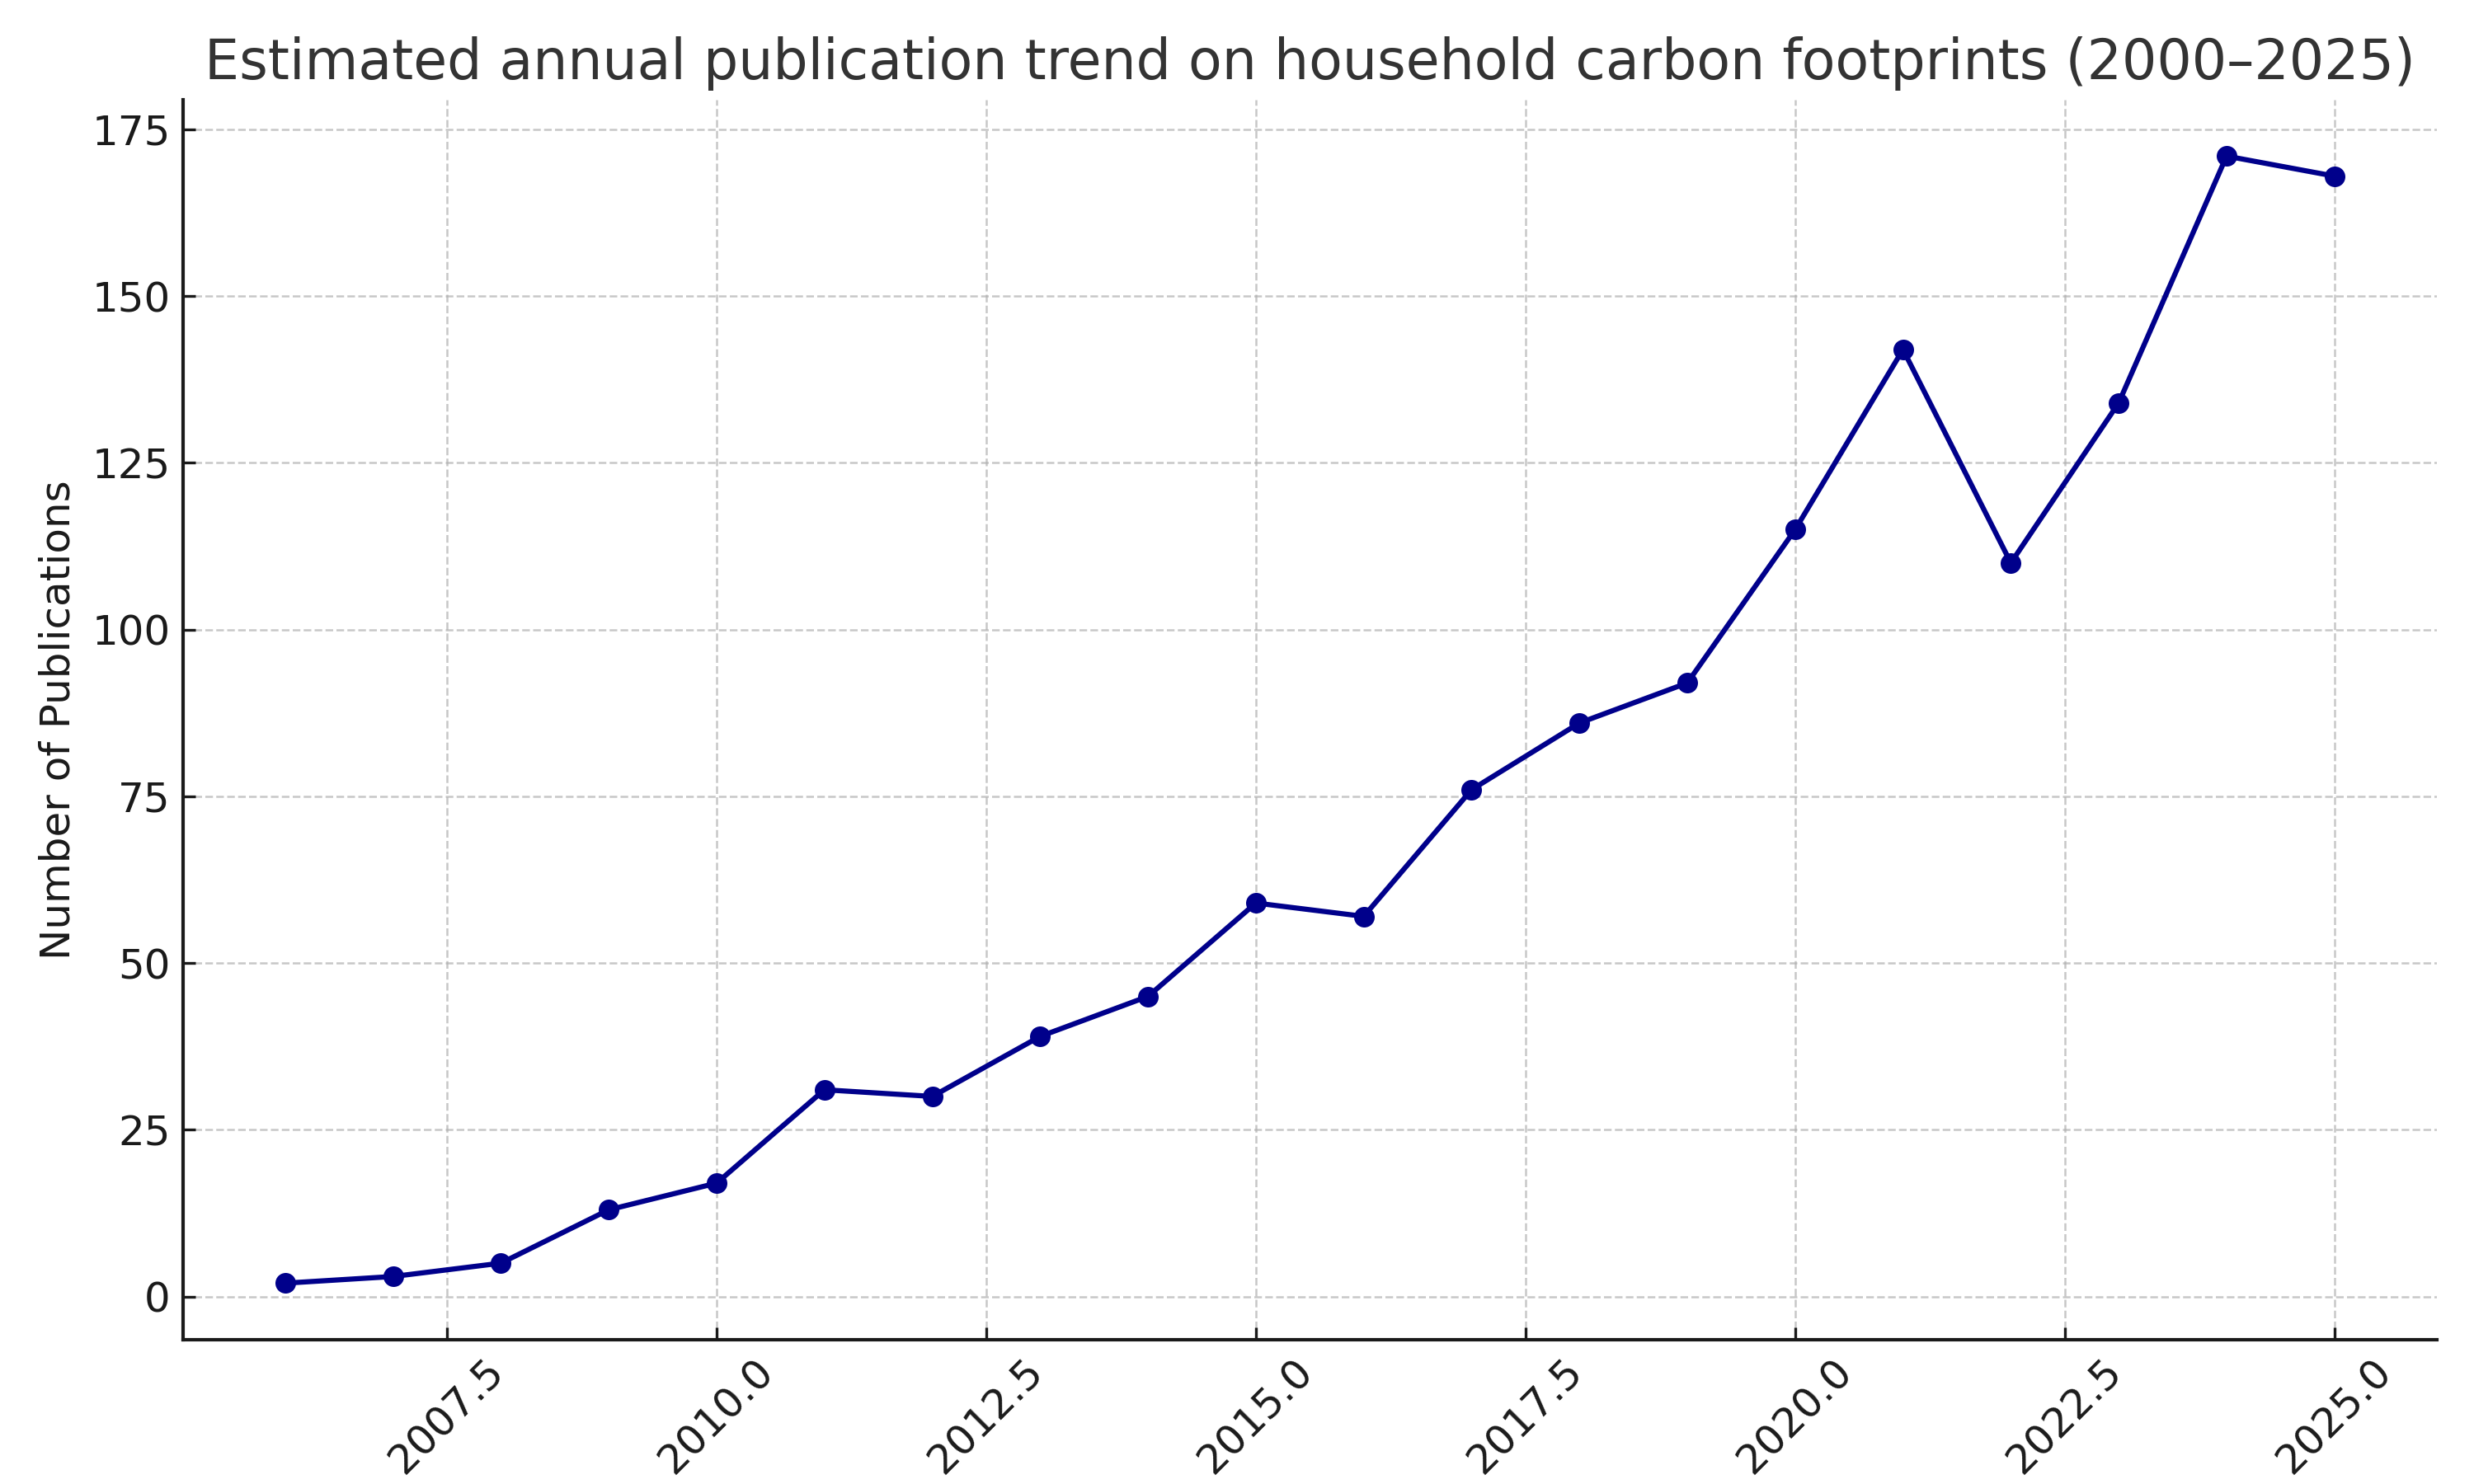
\includegraphics[width=0.85\textwidth]{publication_trend_darkblue_estimated2025.png}
    \caption{\small{Estimated annual publication trend on household carbon footprints (2000–2025). The 2025 value is a linear extrapolation based on mid-year data.}}
\end{figure}

\begin{figure}[htbp]
    \centering
    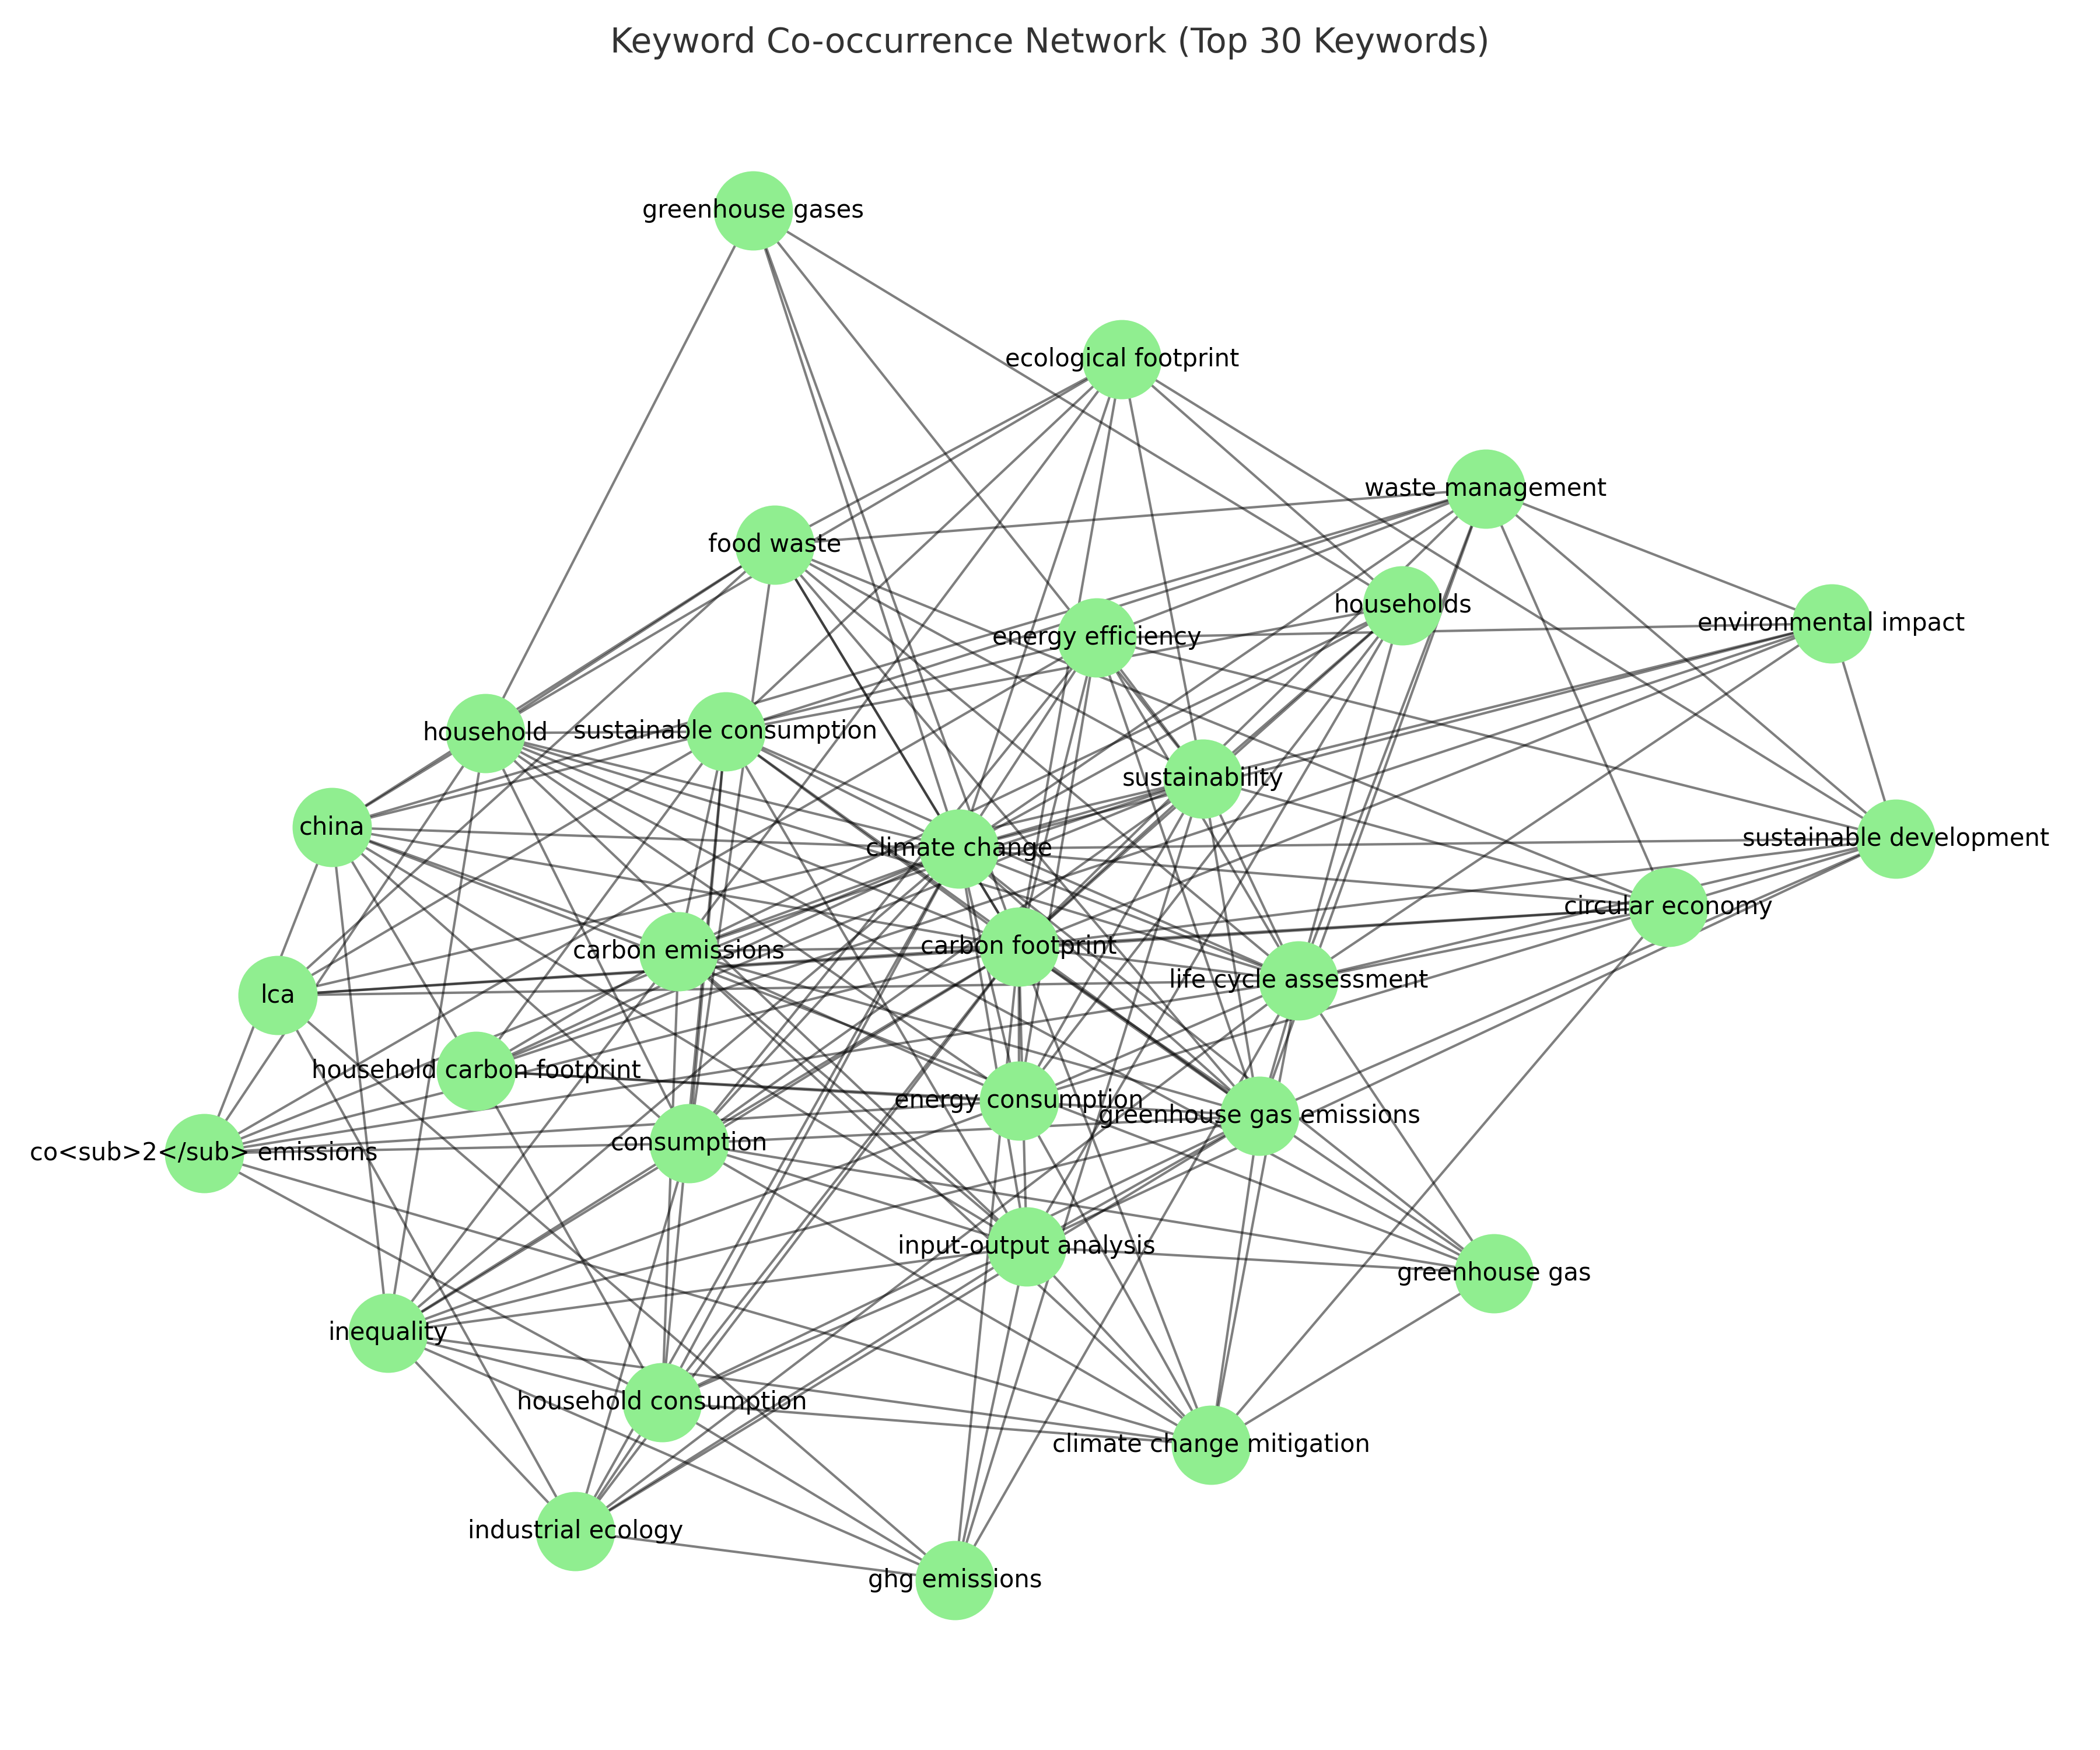
\includegraphics[width=0.85\textwidth]{keyword_cooccurrence.png}
    \caption{\small{Keyword co-occurrence network for the 30 most frequently used terms in household carbon footprint literature (2000–2025).}}
\end{figure}

The estimation of HCF in this literature primarily relies on four methods, chosen here for their widespread use and theoretical distinctiveness—ranging from static, activity-based accounting frameworks (GHG Protocol, LCA, EEIOA) to a market-responsive general equilibrium model (Hakenes and Schliephake) that explicitly captures feedback effects and systemic attribution. The Greenhouse Gas (GHG) Protocol developed by World Resources Institute and the World Business Council for Sustainable Development (WRI and WBCSD, 2004) remains a foundational framework for reporting Scope 1 (direct), Scope 2 (energy-related), and Scope 3 (indirect) emissions. Its activity-based structure, formalized in the IPCC Guidelines (2019), underpins national inventories and has been adapted for household-level analysis---for instance, Weber and Matthews (2008) use expenditure data to allocate emissions across U.S. households. Life Cycle Assessment (LCA) offers a process-based alternative, tracing cradle-to-grave emissions through specific product systems (Guinée, 2011; Steubing et al., 2022), though it often suffers from truncation due to limited system coverage. Environmentally Extended Input-Output Analysis (EEIOA) mitigates this limitation by linking household demand to upstream emissions across sectors (Baiocchi \& Minx, 2010; Wiedmann et al., 2009), and has been further extended to capture spatial disparities in global household emissions (Ivanova et al., 2015).\footnote{Hybrid models have sought to combine the detail of LCA with the coverage of IOA, as in Sonesson et al. (2017) for food systems and in Chard (2024) and Hasegawa et al. (2021) for investment-based emissions.} A recent contribution by Hakenes and Schliephake (2024) introduce a general equilibrium model that endogenizes household consumption and investment, capturing how emissions propagate through price adjustments and market reallocations---thus allowing for a behaviorally grounded and causally consistent attribution of household responsibility.

Despite substantial methodological innovation, critical gaps remain in the literature on household carbon footprint estimation. Emission factor models and life cycle assessment frameworks often treat household preferences and market interactions as exogenous or fixed, limiting their ability to simulate policy-induced behavioral change (Guinée 2011; IPCC 2019). Environmentally extended input-output models, while capable of tracing upstream emissions across global supply chains, typically rely on static technical coefficients and lack behavioral realism in their representation of household decision-making\footnote{See Wiedmann et al. 2009; Ivanova et al. 2015}. Hybrid approaches\footnote{See footnote 6} improve sectoral resolution but generally do not incorporate the endogeneity of prices, income effects, or inter-household spillovers. Moreover, recent studies that examine the carbon intensity of investment portfolios have expanded the scope of household responsibility (Hasegawa et al. 2021), yet often do so in partial equilibrium settings that abstract from feedback effects across markets. The model introduced by Hakenes and Schliephake (2024) addresses many of these limitations by embedding household consumption and investment behavior within a general equilibrium framework. This approach allows for the propagation of individual decisions through price mechanisms and sectoral reallocation, thereby capturing indirect responsibility in a structurally consistent way.

Taken together, the reviewed literature offers a broad but fragmented understanding of HCF accounting and responsibility. While methodological advances have enhanced precision and coverage, questions remain about the causal validity and policy relevance of different approaches. This paper contributes by systematically comparing the four major HCF estimation methods through empirical illustrations and critical evaluation. Beyond methodological comparison, the analysis is motivated by a broader concern: that household-level behavioral change, while symbolically important, offers limited mitigation potential without structural reform on the supply side. As energy and food demands grow with population pressures, the study advocates for shifting the focus of policy design toward upstream interventions in production systems rather than overemphasizing downstream consumption.

\section{Methodology}

This study adopts a comparative and model-based approach to assess the carbon footprints attributable to household consumption and investment behavior. The methodology progresses in three stages: (i) the development of a conceptual framework to analyze carbon accounting methods, (ii) the empirical illustration of the four representative models, and (iii) a comparative evaluation of the normative implications and attribution of responsibility across models. 

The four models considered are: the Greenhouse Gas (GHG) Protocol, Life Cycle Assessment (LCA), Environmentally Extended Input–Output (EEIO) analysis, and the general equilibrium model developed by Hakenes and Schliephake (2024). These methods differ in their conceptual orientation: the GHG Protocol, LCA, and EEIO provide descriptive or accounting-based estimates of emissions tied to observed activities, while the HS model is consequentialist, modeling the systemic effects of household behavior through market mechanisms. 

Each model is implemented using data sources that reflect its underlying methodological logic and disciplinary context. The GHG Protocol combines household consumption expenditure data for Spain in 2022 from Instituto Nacional de Estadística (INE) with emission factors from IPCC guidelines and national energy agencies, enabling scope-based estimation across direct, energy-related, and value chain emissions. The LCA model is presented conceptually rather than empirically, drawing on studies such as Matthews et al. (2008), Peng (2021), and Notarnicola et al. (2017), which illustrate cradle-to-grave emissions accounting for household goods and services. The EEIO model uses household expenditure data from \textit{Eurostat} and spend-based emission factors from \textit{Climatiq.io} (sourced from \textit{EXIOBASE}), covering France, Spain, and Germany for the year 2021. Finally, the general equilibrium model by Hakenes and Schliephake (2024) is implemented using U.S. agricultural sector data, combining wheat production statistics from \textit{USDA}\footnote{The USDA's National Agricultural Statistics Service (NASS) publications provide open data catalogue on U.S. agriculture including crop production, market condition and farm labor.} with sectoral emissions from \textit{FAO} to simulate investor and consumer behavior in a closed economic system. 

The illustrations are intended to highlight how different approaches assign responsibility to households, causality of emissions and reflect varying degrees of abstraction. Rather than pursuing numerical comparability, the analysis foregrounds interpretive contrasts examining how each method conceptualizes the role of households within the broader carbon economy. These methodological divergences form the basis for a normative analysis of climate responsibility, leading to a critical evaluation of the relevance and fairness of household-targeted policy interventions.

\section{The GHG Protocol}
\subsection{Overview of the GHG Protocol}
The Greenhouse Gas (GHG) Protocol is a globally recognized standard for accounting and reporting greenhouse gas emissions. Developed in the late 1990s through a collaboration between the World Resources Institute (WRI) and the World Business Council for Sustainable Development (WBCSD), the GHG Protocol was officially launched in 2001 with the primary aim of providing a consistent and comprehensive framework for emissions accounting across corporate and public sectors. Over the years, its importance has grown significantly, with subsequent expansions such as the development of the GHG Protocol Scope 3 Standard in 2011, which broadened the accounting boundary to include indirect emissions across a company’s value chain. 

The principal reason for employing the GHG Protocol in household-level emissions analysis lies in its capacity to provide a standardized and granular approach to calculating emissions across different dimensions of behavior. It allows for a full inventory of climate impacts arising from everyday life—from fueling a car to investing in equity portfolios. Additionally, the protocol facilitates benchmarking across time and geography, making it possible to compare the carbon intensities of different households or regions. This is particularly valuable for policy-making, where a reliable basis for comparison is needed to design effective incentives, taxes, or subsidy programs aimed at reducing emissions. Moreover, with the rise of ESG (Environmental, Social, and Governance) investing, households are increasingly motivated to assess not only their consumption patterns but also the environmental implications of their financial choices. The GHG Protocol's inclusion of Scope 3 investment-related emissions is thus particularly timely and relevant.

\subsection{Estimation Methodology}

The mathematical formulation under the GHG Protocol for calculating a household’s carbon footprint begins with the aggregation of emissions across three main scopes of emissions. The total carbon footprint of a household is expressed as:

\begin{equation}
CF_{\text{household}} = E_{\text{Scope 1}} + E_{\text{Scope 2}} + E_{\text{Scope 3}}
\end{equation}

Each of these components is calculated based on the product of activity data and corresponding emission factors. For Scope 1, this includes the quantity of fuel combusted in household-controlled devices or vehicles, multiplied by the fuel-specific emission factor. Scope 2 emissions are determined by multiplying electricity or district heating usage by grid-specific emission factors. Scope 3 is more complex and can be further disaggregated into emissions from the consumption of goods and services, and emissions from household investments. For the consumption subcategory, expenditures are multiplied by lifecycle emission factors derived from EEIO models or product-level LCAs. For investment-based emissions, the monetary value of investments is multiplied by portfolio-weighted emission intensities of the respective industries.

\subsection{Application of the GHG Protocol to Spanish Household Data (2022)}

\subsubsection{Data and Implementation}
As an empirical demonstration, the GHG Protocol framework is applied to household expenditure data for Spain in 2022 to illustrate the distribution of emissions across Scopes 1, 2, and 3. The data, sourced from the \textit{Instituto Nacional de Estadística (INE)}, report an average annual household expenditure of €31,568, disaggregated by \textit{COICOP}\footnote{COICOP refers to the Classification of Individual Consumption According to Purpose, a UN standard for categorizing household consumption expenditures. See United Nations Statistics Division (2018).} classification. Spending is allocated across major categories such as housing and energy (32.4\%), food and beverages (16.0\%), and transport (12.0\%), with notable growth in service categories such as restaurants and hotels. This classification facilitates the allocation of lifecycle-based emission factors to each spending category. Emission estimates are calculated by multiplying COICOP-level expenditures with corresponding factors derived from DEFRA and IPCC sources. Energy consumption, reported in gigajoules (GJ) per capita, is also sourced from INE.\footnote{INE (2022), ``Encuesta de Presupuestos Familiares'' and national energy balance data.} A full breakdown is presented in Table A4 (Appendix~A).

\subsubsection{Results and Discussion}
Scope 1 emissions are derived from the direct combustion of fossil fuels by households, primarily through private vehicle use and residential heating. The emission factor associated with petrol is estimated at 73.3 kg CO\textsubscript{2}e/GJ and natural gas at 56.1 kg CO\textsubscript{2}e/GJ. The corresponding calculations are presented in Table 1. Scope 2 emissions refer to indirect emissions associated with the consumption of purchased energy, primarily electricity and district heating, generated externally. In 2022, the average Spanish household consumed approximately 8.96 GJ of heating and cooling energy, with the national electricity grid's emission factor estimated at 92.6 kg CO\textsubscript{2}e per GJ, see Table 2 for the calculations.
% Ensure \usepackage{graphicx} is in your preamble

\begin{table}[h]
\centering
\captionsetup{justification=raggedright,singlelinecheck=false} 
\caption{\small Direct Emissions from Household Energy and Transport (Scope 1)}\label{tab:scope1}
\resizebox{\textwidth}{!}{%
\begin{tabular}{lccc}
\toprule
\textbf{Energy Source} & \textbf{Consumption (GJ/hab)} & \textbf{Emission Factor (kg CO$_2$e/GJ)} & \textbf{Emissions (kg CO$_2$e)} \\
\midrule
Natural Gas (Transport) & 0.04 & 56.1 & 2.24 \\
Petrol (Transport)      & 14.44 & 73.3 & 1058.45 \\
Natural Gas (Heating)   & 0.73 & 56.1 & 40.95 \\
Petrol (Other)          & 0.18 & 73.3 & 13.19 \\
\midrule
\textbf{Total}          &       &       & \textbf{1114.83} \\
\bottomrule
\end{tabular}%
}
\raggedright

\vspace{0.3cm}
\footnotesize{Source: Author's calculations based on INE (2022), DEFRA (2022), and IPCC (2019) emission factors.}
\end{table}


\begin{table}[h]
\centering
\captionsetup{justification=raggedright,singlelinecheck=false} 
\caption{\small Indirect Emissions from Heating and Cooling (Scope 2)}\label{tab:scope2}
\resizebox{\textwidth}{!}{%
\begin{tabular}{lccc}
\toprule
\textbf{Energy Source} & \textbf{Consumption (GJ/hab)} & \textbf{Emission Factor (kg CO$_2$e/GJ)} & \textbf{Emissions (kg CO$_2$e)} \\
\midrule
Heating/Cooling Energy & 8.96 & 92.6 & 829.70 \\
\midrule
\textbf{Total} & & & \textbf{829.70} \\
\bottomrule
\end{tabular}%
}
\raggedright

\vspace{0.3cm}
\footnotesize{Source: Author's calculations based on INE (2022), DEFRA (2022), and IPCC (2019) emission factors.}
\end{table}

Scope 3 emissions represent the most extensive component of the household carbon footprint, capturing the indirect environmental impacts associated with consumption. These emissions encompass the carbon embedded in food, manufactured goods, services, and transport-related infrastructure. For instance, food consumption carries an average emission factor of 0.50 kg CO\textsubscript{2}e per euro, accounting for agricultural production, processing, and distribution. Clothing is assigned a lower factor of 0.25 kg CO\textsubscript{2}e/€, while restaurant services, due to their higher energy intensity, are estimated at 0.40 kg CO\textsubscript{2}e/€. Detailed category-level results for Scope 3 are shown in Table 3.
% Make sure you have \usepackage{booktabs} and \usepackage{graphicx} in your preamble

\begin{table}[h]
\centering
\captionsetup{justification=raggedright,singlelinecheck=false} 
\caption{\small Consumption-Based Emissions (Scope 3)}\label{tab:scope3}
\resizebox{\textwidth}{!}{%
\begin{tabular}{lccc}
\toprule
\textbf{Category} & \textbf{Expenditure (€)} & \textbf{Emission Factor (kg CO$_2$e/€)} & \textbf{Emissions (kg CO$_2$e)} \\
\midrule
Food and non-alcoholic beverages & 5,050 & 0.50 & 2,525.00 \\
Alcoholic beverages and tobacco  &   481 & 0.30 &   144.30 \\
Clothing and footwear            & 1,232 & 0.25 &   308.00 \\
Housing and utilities            &10,243 & 0.25 & 2,560.75 \\
Furnishings                      & 1,296 & 0.30 &   388.80 \\
Health                           & 1,228 & 0.20 &   245.60 \\
Transport services               & 3,794 & 0.30 & 1,138.20 \\
Communications                   &   925 & 0.15 &   138.75 \\
Recreation                       & 1,534 & 0.35 &   536.90 \\
Education                        &   468 & 0.10 &    46.80 \\
Restaurants and hotels           & 2,953 & 0.40 & 1,181.20 \\
Miscellaneous goods and services & 2,364 & 0.30 &   709.20 \\
\midrule
\textbf{Total}                   &        &       & \textbf{9,883.55} \\
\bottomrule
\end{tabular}%
}
\raggedright

\vspace{0.3cm}
\footnotesize{Source: Author's calculations based on INE (2022), DEFRA (2022), and IPCC (2019) emission factors.}
\end{table}

Summing all three scopes, the total annual carbon footprint of a Spanish household in 2022 is estimated at 11,828.08 kg CO\textsubscript{2}e. While Scope 1 and Scope 2 together account for less than 20 \% of the total footprint, largely reflecting fuel use for transport and home energy consumption, Scope 3 alone contributes over four-fifths of total emissions.\footnote{see Table 4} This pattern emphasizes that even households with modest direct energy use can maintain high overall footprints due to the embedded emissions in everyday consumption, pointing to the critical importance of addressing upstream emissions in climate policy.
% Make sure \usepackage{booktabs} is in your preamble

\begin{table}[h]
  \captionsetup{justification=raggedright,singlelinecheck=false} 
\caption{\small Total Household Carbon Footprint by Emission Scopes}\label{tab:total_emissions}
\begin{tabular}{lcccc}
\toprule
 & \small \textbf{Scope 1} & \small \textbf{Scope 2} & \small \textbf{Scope 3} & \small \textbf{Total} \\
\midrule
\small \textbf{Emissions (kg CO$_2$e)} & \small 1,114.83 & \small 829.70 & \small 9,883.55 & \small 11,828.08 \\
 \bottomrule
\end{tabular}

\raggedright

\vspace{0.3cm}
\footnotesize{Source: Author's calculations based on INE (2022), DEFRA (2022), and IPCC (2019) emission factors.}
\end{table}


\subsection{Limitations of the GHG Protocol}

Although widely adopted, the GHG Protocol framework exhibits key limitations when applied to household carbon footprint estimation. Its reliance on average emission factors and static expenditure profiles restricts its capacity to reflect behavioral responses to price signals or policy changes. As evidenced in the Spanish household illustration, Scope 3 emissions constitute the bulk of the footprint, yet the model lacks sensitivity to substitution effects, rebound dynamics, and income elasticity of demand (Hertwich and Peters (2009); Munksgaard et al. (2000)). Furthermore, the use of nationally aggregated emission factors masks regional variability in electricity generation, heating fuels, and consumption infrastructure, potentially distorting footprint estimates in subnational contexts (Lenzen et al. (2004); Wiedmann (2009)).

Enhancing the model with regionally disaggregated data and behavioral elasticities would improve its diagnostic and predictive utility. Incorporating time-series data would further allow for longitudinal assessments of household responses to mitigation policies. Finally, expanding the accounting boundary to include complementary sustainability metrics, such as water use, material intensity, and land footprint, would allow for a more comprehensive assessment of household environmental impacts beyond carbon alone (Wiedmann \& Minx, 2008).

\section{Life Cycle Assessment (LCA)}
\subsection{Overview of the LCA Approach}
The LCA method calculates emissions throughout the entire life cycle of a product or service, from production to disposal. This model captures emissions from every stage of the supply chain and provides a comprehensive assessment of indirect emissions.

The carbon footprint for a single industry using the LCA approach is:
\begin{equation}
   fp_h = q_h \cdot \text{LCA}_j 
\end{equation}

where \(q_h\) is the quantity consumed by household \(h\), and \(\text{LCA}_j\) represents the life cycle emissions per unit in industry \(j\).


\subsection{Estimation Methodology}
This section adapts the framework developed by Peng et al. (2021) to estimate household carbon footprints by combining complementary life cycle assessment (LCA) techniques. Aligned with principles outlined in Guinée (2011) and comparative reviews such as Matthews et al. (2008) and Steubing et al. (2022), the approach quantifies both direct and embodied greenhouse gas (GHG) emissions, together with net carbon sequestration linked to household-level activities.

The methodology integrates three LCA variants to address the system boundary limitations inherent in partial assessments: (1) Process-based LCA is applied to quantify emissions from agricultural operations and livestock production, capturing emissions embedded in material inputs and field-level activities; (2) Input–Output LCA extends the boundary to indirect emissions embedded in household consumption of energy, food, housing, and transport, using environmentally extended input–output (EEIO) tables (Weber and Matthews, 2008); (3) Hybrid LCA bridges both levels by combining process inventory detail with macroeconomic input–output linkages, reducing truncation errors and capturing carbon flows related to afforestation, durable goods, and other land-use changes (Crawford et al., 2018; Shen et al., 2023).

Following Peng et al. (2021), the model distinguishes five core domains: direct energy use, short-lived and durable consumption, household agriculture, afforestation, and livestock management. Activity-specific emissions are parameterized using survey-derived data and regionally adjusted emission factors in accordance with IPCC (2019) guidelines. This combined accounting framework quantifies net household carbon flows as the balance of annual GHG emissions and sequestration within a unified system boundary:

\begin{equation}
CF_i = \sum_{n} E_{in} + \sum_{m} S_{im}
\end{equation}
where $CF_i$ represents the Carbon footprint of household $i$, $E_{in}$ is the annual carbon emissions of household $i$ in category $n$ and $S_{im}$ is the annual carbon sequestration of household $i$ in category $m$. This disaggregated yet integrated structure provides the basis for the following activity-specific equations, which formally express how annual household emissions and sequestration are calculated within each functional domain.

\subsubsection{Carbon Emissions from Direct Energy Consumption}
The emissions from household direct energy use are estimated by multiplying the quantity of fuel consumed by its corresponding emission factor. For each household $i$, the total emissions attributable to direct fuel combustion denoted by $E_{id}$ is calculated as:
\begin{equation}
E_{id} = \sum_d (F_{id} \cdot EF_d)
\end{equation}
where $F_{id}$ denotes the annual consumption of household $i$  for fuel type $d$. The fuel-specific emission factor $EF_{d}$ combines oxidation efficiency, fuel composition, and calorific value, consistent with IPCC (2019) guidelines:
\begin{equation}
EF_d = OX_d \cdot \left(C_{o,d} \cdot \frac{12}{44} + C_{h,d} \cdot \frac{12}{16}\right) \cdot H_d \cdot 10^{-9}
\end{equation}
Here, $OX_d$ represents the oxidation efficiency, typically assumed to be 100\% for complete combustion; $C_{o,d}$ and $C_{h,d}$ are the fuel-specific emission coefficients for CO$_2$ and CH$_4$, respectively; and $H_d$ denotes the net calorific value of the fuel. The conversion factors ensure that carbon content is expressed in consistent units of tonnes CO$_2$ equivalent per unit of fuel input.

\subsubsection{Carbon Emissions from Living Consumption}

Emissions attributable to household consumption of goods and services are divided into two categories: short-lived products and durable consumer goods. The total annual emissions from short-lived consumption are given by:

\begin{equation}
E_{if} = \sum_f (EF_f \cdot C_{if})
\end{equation}

where $E_{if}$ denotes the annual carbon emissions from short-lived good $f$, $C_{if}$ is the quantity of product $f$ consumed by household $i$, and $EF_f$ is its corresponding life cycle emission factor. For durable consumer products, the embodied emissions are amortized over the product's expected service life to obtain an annualized footprint:

\begin{equation}
E_{ij} = \sum_j \frac{(EF_j \cdot C_{ij})}{L_j}
\end{equation}

Here, $E_{ij}$ represents the annual emissions associated with durable product $j$, $C_{ij}$ is the total quantity purchased, $EF_j$ is the relevant life cycle emission factor, and $L_j$ is the product’s average lifetime (in years). This treatment ensures that emissions embedded in capital household goods are allocated proportionally across their period of use, consistent with standard LCA accounting conventions.


\subsubsection{Carbon Footprint in Agricultural Activities}

Emissions and sequestration associated with household-level agricultural production are accounted for through inputs, on-site operations, and net biomass growth. The total annual carbon footprint from agricultural activities for household $i$ is calculated as:

\begin{equation}
CF_{ia} = \sum_a (EF_a \cdot M_{ia}) + \sum_t (EF_t \cdot FS_{ia}) + \sum_v (B_v \cdot 0.475)
\end{equation}

Here, $CF_{ia}$ denotes the net carbon impact of agricultural activities. $M_{ia}$ represents the quantity of material input $a$ (such as fertilizers or pesticides) applied by household $i$, with an associated emission factor $EF_a$. The second term accounts for emissions from field operations, where $FS_{ia}$ is the cultivated field size and $EF_t$ is the emission factor per unit area for operation $t$ (e.g., tillage, irrigation). The final term reflects the carbon sequestered in above-ground biomass, with $B_v$ indicating the dry biomass yield for crop or vegetation type $v$, multiplied by a standard carbon content coefficient of 47.5\% (IPCC default for plant biomass).


\subsubsection{Carbon Sequestration from Afforestation}

Carbon sequestration through household-level afforestation is estimated based on the area of land dedicated to tree planting and the average carbon stock of the tree species established. The annual sequestration from afforestation for household $i$ is given by:

\begin{equation}
S_{iaf} = FS_{iaf} \cdot CS_{\text{citrus}}
\end{equation}

In this expression, $S_{iaf}$ represents the amount of carbon sequestered through afforestation activities, $FS_{iaf}$ denotes the field size (in hectares) allocated for tree planting by household $i$, and $CS_{\text{citrus}}$ is the mean carbon stock per unit area for citrus trees or other comparable species. The carbon stock factor reflects the average annual carbon uptake, accounting for biomass accumulation under local growth conditions.


\subsubsection{Carbon Emissions from Livestock Raising}

Emissions from household livestock activities include fodder production, enteric fermentation, and manure management. The total annual emissions from livestock raising for household $i$ are calculated as:

\begin{equation}
E_{il} = \sum_f (EF_{if} \cdot F_{if}) + \sum_l (EF_{il} \cdot N_{il})
\end{equation}

In this formulation, $E_{il}$ represents the total carbon emissions attributable to livestock-related activities. $F_{if}$ denotes the annual quantity of fodder consumed by livestock, multiplied by the corresponding emission factor $EF_{if}$ to account for upstream impacts of fodder cultivation and transport. The second term captures direct emissions from livestock, where $N_{il}$ is the number of animals of type $l$ and $EF_{il}$ is the per-animal emission factor, which includes methane emissions from enteric fermentation and nitrous oxide from manure management.



\subsubsection{Aggregate Formula for Household Carbon Footprint}

The total household carbon footprint ($CF_{\text{total}}$) aggregates emissions and sequestration from direct energy use, living consumption, agricultural production, afforestation, and livestock raising, as specified in Equations (4) to (10).

\begin{align}
CF_{\text{total}} = & \underbrace{\sum_d \left(F_{id} \cdot EF_d\right)}_{\text{Direct energy}} + 
\underbrace{\sum_f \left(EF_f \cdot C_{if}\right) + \sum_j \frac{\left(EF_j \cdot C_{ij}\right)}{L_j}}_{\text{Living consumption}} \nonumber \\
& + \underbrace{\sum_a \left(EF_a \cdot M_{ia}\right) + \sum_t \left(EF_t \cdot FS_{ia}\right) + \sum_v \left(B_v \cdot 0.475\right)}_{\text{Agriculture}} \nonumber \\
& - \underbrace{\sum_{iaf} \left(FS_{iaf} \cdot CS_{\text{citrus}}\right)}_{\text{Afforestation}} +
\underbrace{\sum_f \left(EF_{if} \cdot F_{if}\right) + \sum_l \left(EF_{il} \cdot N_{il}\right)}_{\text{Livestock}}.
\label{eq:aggregate}
\end{align}

By integrating disaggregated activity data with region-specific emission factors, this aggregate formulation is a consistent representation of the net annual GHG balance at the household level, consistent with best practices in household carbon accounting (Ivanova et al., 2016; Dubois et al., 2019). 

Beyond its measurement function, this structure highlights how household decisions on energy use, consumption patterns, and land management jointly influence emissions outcomes (Hertwich and Peters, 2009). Such clarity enables scenario analysis of behavioral shifts and technological choices, informing targeted interventions like carbon price adjustments, renewable energy adoption incentives, or compensation for sequestration through land-based measures (Rogelj et al., 2018; Steubing et al., 2022). As shown in recent household-level studies, aligning micro-level incentives with broader climate objectives is essential to internalize externalities and realize cost-effective emission reductions (Wiedmann et al., 2020).

\subsection{Empirical Findings from LCA Studies}

An integrated life cycle assessment (LCA) illustration clarifies how the total household carbon footprint, as defined by Equations (4) to (10), is distributed across major activity domains and is illustrated in Figure 3. Drawing on estimates from Peng et al.\ (2021), Notarnicola et al.\ (2017), and Matthews et al.\ (2008), direct household energy use, including heating fuels and private vehicle fuels, accounts for approximately 20\% to 30\% of total greenhouse gas emissions. Living consumption, which covers short-lived goods, food purchases, and services, represents the largest share at about 50\% to 60\%. Durable goods, including household appliances and furniture, add an additional 5\% to 10\% of total emissions when annualized, showing the relevance of product lifespan and embedded material flows. 

Together, this evidence shows that focusing only on direct household fuel use underestimates the total climate impact of residential lifestyles because indirect emissions embedded in goods and services account for most impacts, as discussed by Hertwich and Peters (2009). A comprehensive, activity-based LCA offers a more realistic basis for identifying mitigation options such as improving building energy performance, extending product lifespans, sourcing materials more sustainably, and investing in land-based carbon sequestration. This broader perspective supports the development of household-level strategies that address systemic drivers of emissions rather than isolating individual consumption categories.


\begin{figure}[h]
\centering
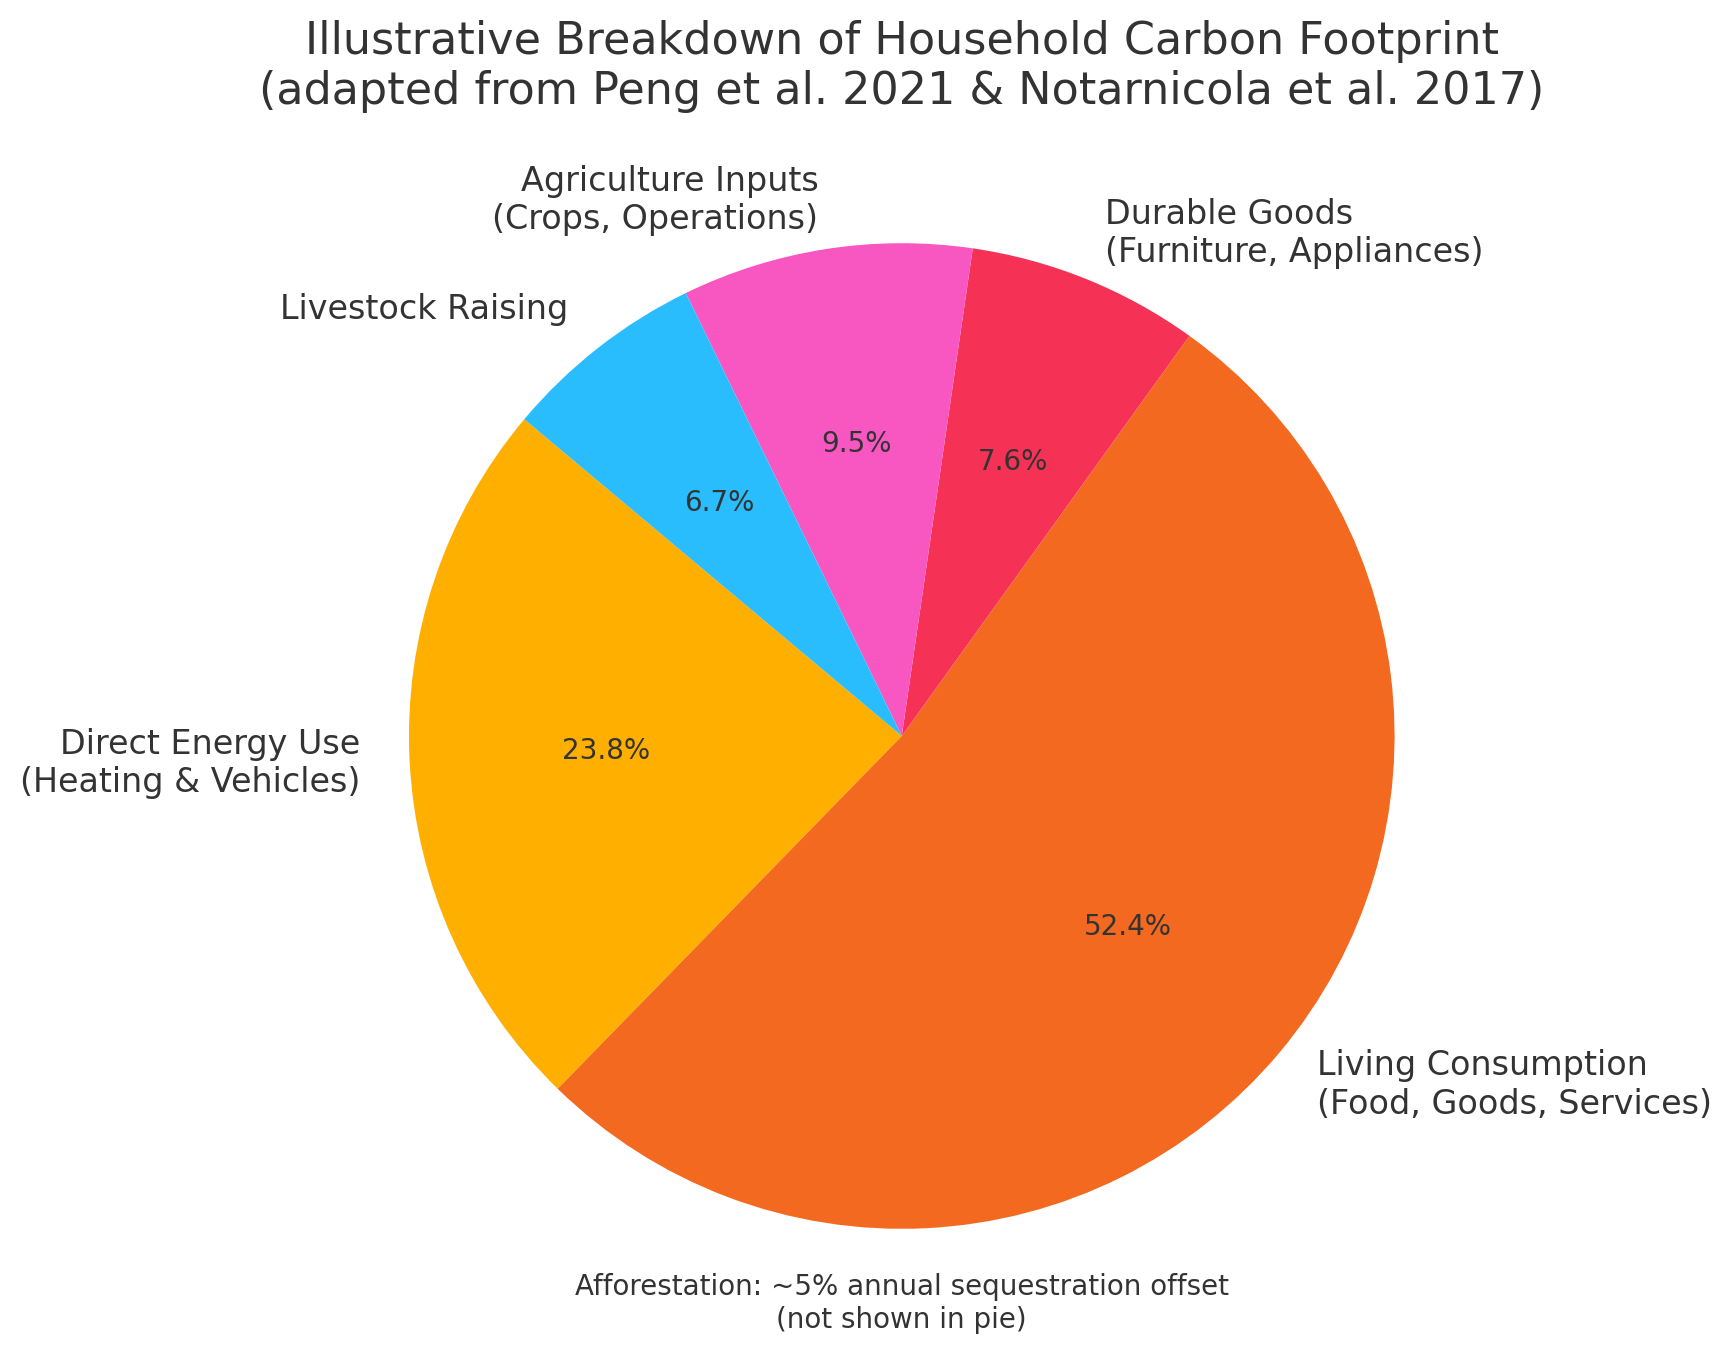
\includegraphics[width=0.8\linewidth]{LCA_pie.png}
\small \caption{Relative contribution of household activities to carbon footprint based on an integrated LCA approach. Findings are adapted from Peng et al.\ (2021), Notarnicola et al.\ (2017), and Matthews et al.\ (2008).}
\end{figure}

\section{Input–Output Model and Carbon Footprint Estimation}
The environmentally extended Input-Output (EEIO) framework provides a macroeconomic approach for quantifying household carbon footprints by tracing both direct and upstream greenhouse gas (GHG) emissions embedded in goods and services. 

\subsection{Leontief Input–Output Framework}

\subsubsection{Input–Output Identity}

We begin with the standard Leontief system, where total output \( \mathbf{X} \) is the sum of intermediate input requirements and final demand:

\begin{equation}
\mathbf{X} = \mathbf{A} \mathbf{X} + \mathbf{F}.
\end{equation}

Solving for total output yields the fundamental input–output identity:

\begin{equation}
\mathbf{X} = {(\mathbf{I} - \mathbf{A})}^{-1} \mathbf{F}.
\end{equation}

Here, \( \mathbf{A} \) is the technical coefficient matrix, \( \mathbf{F} \) is the vector of household final demand, and \( {(\mathbf{I} - \mathbf{A})}^{-1} \) is the Leontief inverse, which accounts for the total production required (both direct and indirect) to satisfy final demand.

\subsubsection{Technical Coefficient Matrix}

Each element \( A_{ij} \) of the matrix \( \mathbf{A} \) is defined as:

\begin{equation}
A_{ij} = \frac{z_{ij}}{x_j},
\end{equation}

where \( z_{ij} \) denotes the monetary value of inputs from sector \( i \) to sector \( j \), and \( x_j \) is the total output of sector \( j \). The matrix \( \mathbf{A} \) reflects the technological input structure of the economy.

\subsubsection{Stability of the Leontief Inverse}

The Leontief inverse \( {(\mathbf{I} - \mathbf{A})}^{-1} \) exists and is finite if the matrix \( \mathbf{A} \) satisfies the stability condition \( \rho(\mathbf{A}) < 1 \), where \( \rho(\cdot) \) denotes the spectral radius (i.e., the largest absolute eigenvalue). This condition ensures that the production system is productive and does not require infinite inputs. In applied input--output tables, a sufficient (but not necessary) condition is that the column sums of \( \mathbf{A} \) are each less than one:
\[
\sum_i A_{ij} < 1 \quad \text{for all } j.
\]
This implies that each sector uses less than one unit of intermediate input to produce one unit of output, a condition that is generally satisfied in empirical datasets (Miller and Blair, 2009). A numerical illustration of the stability condition, along with matrix-based examples and emission multiplier computation, is provided in Appendix B.

\subsubsection{Carbon Footprint Estimation via Input–Output Modelling}

The environmentally extended input–output (EEIO) model estimates household carbon footprints by applying sectoral emission intensities to the total output vector required to satisfy final demand:

\begin{equation}
\mathbf{E} = \mathbf{C} {(\mathbf{I} - \mathbf{A})}^{-1} \mathbf{F},
\end{equation}

where \( \mathbf{C} \) is the vector of direct emission intensities (e.g., kg CO\textsubscript{2}e per euro of output), and \( \mathbf{E} \) is the resulting emissions attributable to household consumption. This formulation captures both direct and upstream (supply chain) emissions associated with consumption.

\paragraph{Tiered Decomposition of Household Emissions:}

Following Matthews et al.~(2008) and Long et al.~(2019), the total household footprint can be analytically decomposed into three tiers:

\paragraph{Tier 1: Direct Emissions}

\begin{equation}
\mathbf{E}_1 = \mathbf{C}_d \cdot \mathbf{F}_d,
\end{equation}

where \( \mathbf{F}_d \) is household consumption of directly combusted fuels and \( \mathbf{C}_d \) is the corresponding emission intensity vector.

\paragraph{Tier 2: Indirect Energy Emissions}

\begin{equation}
\mathbf{E}_2 = \mathbf{C}_e \cdot {(\mathbf{I} - \mathbf{A})}^{-1} \cdot \mathbf{F}_e,
\end{equation}

with \( \mathbf{F}_e \) representing consumption of electricity and district heating, and \( \mathbf{C}_e \) their emission intensities.

\paragraph{Tier 3: Indirect Supply Chain Emissions}

\begin{equation}
\mathbf{E}_3 = \mathbf{C} \cdot {\left[(\mathbf{I} - \mathbf{M})(\mathbf{I} - \mathbf{A})\right]}^{-1} \cdot \left[(\mathbf{I} - \mathbf{M}) \cdot \mathbf{F} + \mathbf{EX} \right],
\end{equation}

where \( \mathbf{M} \) is a diagonal matrix of sectoral import shares, and \( \mathbf{EX} \) accounts for exports. This import-adjusted EEIO formulation ensures emissions are assigned to domestic demand (Long et al., 2019; Sheng et al., 2024).
 
\paragraph{The Total Household Footprint}

\begin{equation}
    \mathbf{E}_{\text{total}} = \mathbf{E}_1 + \mathbf{E}_2 + \mathbf{E}_3.
\end{equation}

where \( \mathbf{E}_{\text{total}} \) represents the total household carbon footprint, capturing all direct and indirect emissions associated with household consumption.
This integrated EEIO framework mitigates truncation and boundary errors typical of process-based LCA, capturing the full feedback loops of modern economies (Matthews et al., 2008; Steubing et al., 2022).


\subsection{Empirical Illustration of the Input-Output Model}

In this illustration, pre-calculated environmentally extended emission intensities (kg CO$_{2}$e per euro spent) are applied to household consumption data for France, Spain, and Germany for 2021. These intensities represent the aggregated effect of $\mathbf{C} {(\mathbf{I}-\mathbf{A})}^{-1}$ and are derived from the EXIOBASE multi-regional input-output (MRIO) model, as accessed via Climatiq.io.\footnote{These coefficients implicitly incorporate trade-adjusted upstream emissions, though no explicit import share matrix was applied in this illustration.} The method aligns with the tier-3 comprehensive accounting approach discussed in Matthews et al.~(2008), Long et al.~(2019), and Sheng et al.~(2024).

\subsubsection{Data and Methodology}

The Leontief inverse ${(\mathbf{I} - \mathbf{A})}^{-1}$ then expands final demand to include both direct and indirect production requirements.

\begin{equation}
  EF_i = \sum_{j} C_j L_{ji}, 
\quad \text{where} \quad 
L = {(\mathbf{I} - \mathbf{A})}^{-1}.
\end{equation}



Here, $C_j$ denotes the direct emissions intensity for producing sector $j$, and $L_{ji}$ represents the total requirements linking producing sectors $j$ and $i$. The resulting spend-based factors are published through Climatiq.io, which provides up-to-date coefficients aggregated from EXIOBASE under a permissive data license \footnote{Creative Commons Attribution-ShareAlike 4.0 International License}.

To ensure numerical stability, EXIOBASE balances its input-output tables using harmonised supply-use statistics, preventing divergence in the Leontief inverse. An additional feasibility check confirms that the sum of each column in $\mathbf{A}$ remains below unity, preserving the productive structure required for invertibility.

Annual household final consumption expenditure for France, Spain, and Germany was sourced from Eurostat for the year 2021 and harmonised to euros at the average annual exchange rate. For each expenditure category $i$ and country $c$, the household carbon footprint is estimated by multiplying the national expenditure by the corresponding spend-based factor:

\begin{equation}
  E_{i,c} = F_{i,c} \times EF_i.
\end{equation}

For instance, for France, the estimated annual household spending on food and non-alcoholic beverages is approximately

\[
F_{\text{food,FR}} = 1.322 \times 10^9 \times 0.139 = 183.8 \times 10^9~\text{EUR}.
\]

Multiplying this by the category-specific factor of 0.48~kg CO$_2$e per euro yields an estimated

\[
E_{\text{food,FR}} = 183.8 \times 10^9 \times 0.48 = 88.2 \times 10^6~\text{tonnes CO}_2\text{e}.
\]

The same procedure is applied across all final demand categories and for Spain and Germany. This method follows the tier-3 EEIO approach and systematically allocates upstream supply chain emissions, providing a comprehensive perspective on the consumption-driven climate impact of households. All emission factors are listed in Appendix~A, Table~A5.

\subsubsection{Results}

Table 5 summarizes the estimated household carbon footprints for France, Spain, and Germany in 2021, derived using the environmentally extended input--output model. The full breakdown by expenditure category is reported in Appendix~A (Tables~A6--A8).

\begin{table}[h]
 \captionsetup{justification=raggedright,singlelinecheck=false} 
\caption{\small{Total estimated household carbon footprints (2021)}}
\begin{tabular}{lcc}
\toprule
\textbf\small{Country} & \textbf\small{Expenditure (bn €)} & \textbf\small{Emissions (Mt CO\textsubscript{2}e)} \\
\midrule
\small France & \small 1322.0 & \small 420.0 \\
\small Spain & \small 747.9 & \small 227.0 \\
\small Germany & \small 1794.8 & \small 545.9 \\
\bottomrule
\end{tabular}
\raggedright

\vspace{0.3cm}
\footnotesize{Source: Author's calculations based on Eurostat 2021 data on Household final consumption expenditure by purpose (COICOP 1999) and EXIOBASE (2025) emission factors.}
\end{table}

In all three countries, the dominant drivers of household emissions are housing, food, and transport. These sectors together account for over 60\% of the footprint, reflecting the carbon intensity of residential energy use, agri-food supply chains, and private mobility. The relative magnitude and structure of results are consistent with earlier multi-regional IO studies (Matthews et al.~2008; Long et al.~2019; Sheng et al.~2024), confirming the utility of EEIO methods for policy-relevant footprint accounting.

Thus, the footprint estimates capture the sectoral and cross-country variation in household carbon intensity, illustrating the effectiveness of the EEIO approach in quantifying consumption-driven emissions at national scale.


\subsection{Comparative Assessment of LCA and EEIOA for Household Carbon Footprint Estimation}

Life cycle assessment (LCA) and environmentally extended input--output analysis (EEIOA) are both established approaches for estimating household carbon footprints but differ in system boundaries and detail. LCA quantifies emissions by summing process-based impacts across all life cycle stages, often including capital goods and infrastructure explicitly.

In this illustration, the household carbon footprint is quantified using an LCA framework adapted from Steubing et al.~(2022). The structure of the total footprint, previously defined in Equation~(11), can be re-stated as:

\begin{equation}
\text{CF}_{\text{total}} = \sum_d (F_{id} \cdot EF_d) 
+ \sum_f (C_{if} \cdot EF_f) 
+ \sum_j \left( \frac{C_{ij} \cdot EF_j}{L_j} \right)
+ \sum_a (M_{ia} \cdot EF_a)
- \sum_t (S_{it} \cdot CS_t).
\end{equation}
where fuel use, short-lived and durable goods, capital goods lifespan, material inputs, and carbon stock changes are all explicitly accounted for.

In comparison, the EEIOA model, as defined in Equation~(15), estimates the footprint as:

\begin{equation}
\text{CF}_{\text{EEIOA}} = {C (I - A)}^{-1} F.
\end{equation}

In standard practice, the final demand vector $F$ typically excludes gross fixed capital formation, meaning that capital goods for future production are not fully reflected in the EEIOA results. This distinction explains why LCA-based footprints can exceed EEIOA estimates in capital-intensive sectors. Steubing et al.~(2022) demonstrate that for electricity, fossil-based power systems show close agreement between LCA and EEIOA estimates, whereas renewable electricity systems diverge more significantly due to the inclusion of construction and infrastructure impacts in the LCA boundary.

This comparative perspective highlights that LCA captures emissions from long-lived assets more comprehensively, while EEIOA better reflects systemic supply chain emissions embedded in everyday household expenditure. Using both approaches together clarifies how immediate consumption interacts with infrastructure and capital investment to shape total household carbon footprints.

\section{The Hakenes \& Schliephake Model}

Traditional methods for estimating household carbon footprints attribute emissions based on direct consumption or financial ownership in emitting industries. However, they often ignore the market feedback loops triggered by individual decisions — such as how a household reducing demand might simply shift that demand to other consumers or investors.

The model developed by Hakenes and Schliephake (2024) addresses this issue through a general equilibrium framework. By embedding both product and financial markets, the model assigns carbon footprints based not only on what households consume or invest in, but also on the spillover effects of those choices across the economy. This consequentialist approach attempts to capture the true marginal impact of household behavior on aggregate emissions.

\subsection{Deriving the Household Footprint in a One-Industry Economy}

This paper considers a simplified version of the Hakenes and Schliephake (2024) model in a one-industry setting. A representative homogeneous good is produced using capital as the only input. Firms operate under constant returns to scale, and the marginal cost of production is denoted by $c$.

\subsubsection{Production and Emissions}

Let $Q$ denote the total output produced and consumed in the economy, and $I$ the total investment in capital. With linear technology:
\begin{equation}
I = cQ 
\end{equation}

Each unit of output causes emissions $x$, so total emissions in the economy are:
\begin{equation}
X = xQ 
\end{equation}

\subsubsection{Firms and Capital Market}

Firms raise capital $I$ from households, produce $Q$, and sell output at price $P$. Investors are repaid with:
\begin{equation}
r = \frac{P}{c} + \lambda + \varepsilon 
\end{equation}
where $\lambda$ is the deterministic liquidation value and $\varepsilon \sim \mathcal{N}(0, \sigma^2)$ is a noise term. In competitive equilibrium, expected profits are zero.

\subsubsection{Household Optimization Problem}

Household $h$ has wealth $w$ and allocates it between consumption $q_h$ and investment $i_h$. The residual earns the risk-free return $r_f$:
\begin{equation}
m_h = r i_h + r_f(w - i_h) - P q_h 
\end{equation}

Utility depends on consumption, terminal wealth, and disutility from global emissions:
\begin{equation}
U_h = \mathbb{E} \left[ -e^{-\alpha \left( a q_h - \frac{b}{2}q_h^2 + m_h - xQ \right)} \right] \tag{5}
\end{equation}

Substituting $m_h$ into the utility function and using properties of the exponential-normal form yields:
\begin{equation}
\mathbb{E}[U_h] = -\exp\left\{ -\alpha \left[ (a - P)q_h - \frac{b}{2}q_h^2 + r_f w + \left( \frac{P}{c} + \lambda - r_f \right)i_h - \frac{\alpha}{2}\sigma^2 i_h^2 - xQ \right] \right\} 
\end{equation}

\subsubsection{First-Order Conditions}

Maximizing utility leads to:
\begin{align}
\frac{\partial \mathbb{E}[U_h]}{\partial q_h} = 0 &\Rightarrow a - x - b q_h - P = 0 \Rightarrow q_h = \frac{a - x - P}{b} \\
\frac{\partial \mathbb{E}[U_h]}{\partial i_h} = 0 &\Rightarrow \frac{P}{c} + \lambda - r_f - \alpha \sigma^2 i_h = 0 \Rightarrow i_h = \frac{1}{\alpha \sigma^2}\left( \frac{P}{c} + \lambda - r_f \right) 
\end{align}

\subsubsection{Market Equilibrium and Derivation of the Weighting Parameter}

Let $q_{-h}$ and $i_{-h}$ be the consumption and investment of any other household. In equilibrium with $n$ households:
\begin{equation}
Q = q_h + (n - 1)q_{-h}, \quad I = i_h + (n - 1)i_{-h}, \quad I = cQ 
\end{equation}

From the FOCs of other households:
\begin{align}
q_{-h} &= \frac{a - x - P}{b}, \\
i_{-h} &= \frac{1}{\alpha \sigma^2} \left( \frac{P}{c} + \lambda - r_f \right) 
\end{align}

Then total investment is:
\begin{equation}
I = (n - 1)i_{-h} = \frac{n - 1}{\alpha \sigma^2} \left( \frac{P}{c} + \lambda - r_f \right)
\end{equation}

Substituting into $Q = I/c$:
\begin{equation}
Q = \frac{n - 1}{c \alpha \sigma^2} \left( \frac{P}{c} + \lambda - r_f \right) 
\end{equation}

Solving for $P$ gives the supply curve:
\begin{equation}
P = c(r_f - \lambda) + \frac{c^2 \alpha \sigma^2}{n - 1} Q 
\end{equation}

From Eq. (29), the demand of the $n - 1$ households is:
\begin{equation}
q_{-h} = \frac{a - x - P}{b} \Rightarrow Q = q_h + (n - 1)\cdot \frac{a - x - P}{b} 
\end{equation}

Solving Eqs. (36) and (37) simultaneously for $Q$ as a function of $q_h$ and $i_h$ gives:
\begin{equation}
Q = (n - 1) \cdot \frac{a - x - c(r_f - \lambda)}{b + c^2 \alpha \sigma^2} + \phi q_h + (1 - \phi) \cdot \frac{i_h}{c} 
\end{equation}
where:
\begin{equation}
\phi = \frac{b}{b + c^2 \alpha \sigma^2} 
\end{equation}

\subsubsection{Household Footprint}

The consequentialist footprint is defined as the marginal impact of household $h$ on total emissions:
\begin{align}
fp_h &= x \cdot (Q(q_h, i_h) - Q(0, 0)) \\
&= x \left( \phi q_h + (1 - \phi) \cdot \frac{i_h}{c} \right) 
\end{align}

When $\sigma^2 = 0$, $\phi = 1$ and the entire footprint is consumption-driven. When $b = 0$, $\phi = 0$ and the footprint is investment-driven.

This decomposition ensures that total emissions are fully accounted for:
\begin{equation}
\sum_h fp_h = xQ = X 
\end{equation}

\subsubsection{Comparative Statics of the Weighting Parameter \( \boldsymbol{\phi} \)}

This section investigates how the footprint weighting parameter \( \boldsymbol{\phi} \), defined as
\[
\boldsymbol{\phi} = \frac{b}{b + c^2 \alpha \sigma^2},
\]
responds to changes in the underlying structural parameters of the model.

Differentiating \( \boldsymbol{\phi} \) with respect to the coefficient of absolute risk aversion \( \alpha \), we obtain
\[
\frac{\partial \boldsymbol{\phi}}{\partial \alpha} = -\frac{b c^2 \sigma^2}{{(b + c^2 \alpha \sigma^2)}^2} < 0.
\]
This implies that as households become more risk-averse, the footprint share attributed to consumption declines, while the relative importance of investment decisions increases.

With respect to the volatility of financial returns, captured by \( \sigma^2 \), we find
\[
\frac{\partial \boldsymbol{\phi}}{\partial \sigma^2} = -\frac{b c^2 \alpha}{{(b + c^2 \alpha \sigma^2)}^2} < 0.
\]
An increase in financial risk similarly reduces \( \boldsymbol{\phi} \), shifting the footprint burden from consumption to investment channels.

Finally, consider the effect of changing the curvature of the utility function through the parameter \( b \). Differentiation yields
\[
\frac{\partial \boldsymbol{\phi}}{\partial b} = \frac{c^2 \alpha \sigma^2}{{(b + c^2 \alpha \sigma^2)}^2} > 0.
\]
A higher value of \( b \), indicating stronger diminishing marginal utility from consumption, increases the share of the footprint attributed to consumption activities.

In sum, the weighting parameter \( \boldsymbol{\phi} \) is decreasing in both risk aversion and return volatility, and increasing in the concavity of consumption preferences. These results highlight how the relative responsibility of consumption and investment for carbon emissions is endogenous to household behavior and financial risk, making the model responsive to empirical variation across households or economies.

\subsection{Empirical Illustration: Application of the Single-Industry Model}

\subsubsection{Data and Methodology}
Here, the simplified version of the Hakenes and Schliephake (2024) model is applied to the U.S. wheat market, using USDA data from 2010 to 2017\footnote{See Table A9 in Appendix A}. Production volumes serve as a proxy for quantity supplied, while total domestic use approximates quantity demanded. Farm prices are taken as observed average annual prices.

\begin{figure}[ht]
    \centering
    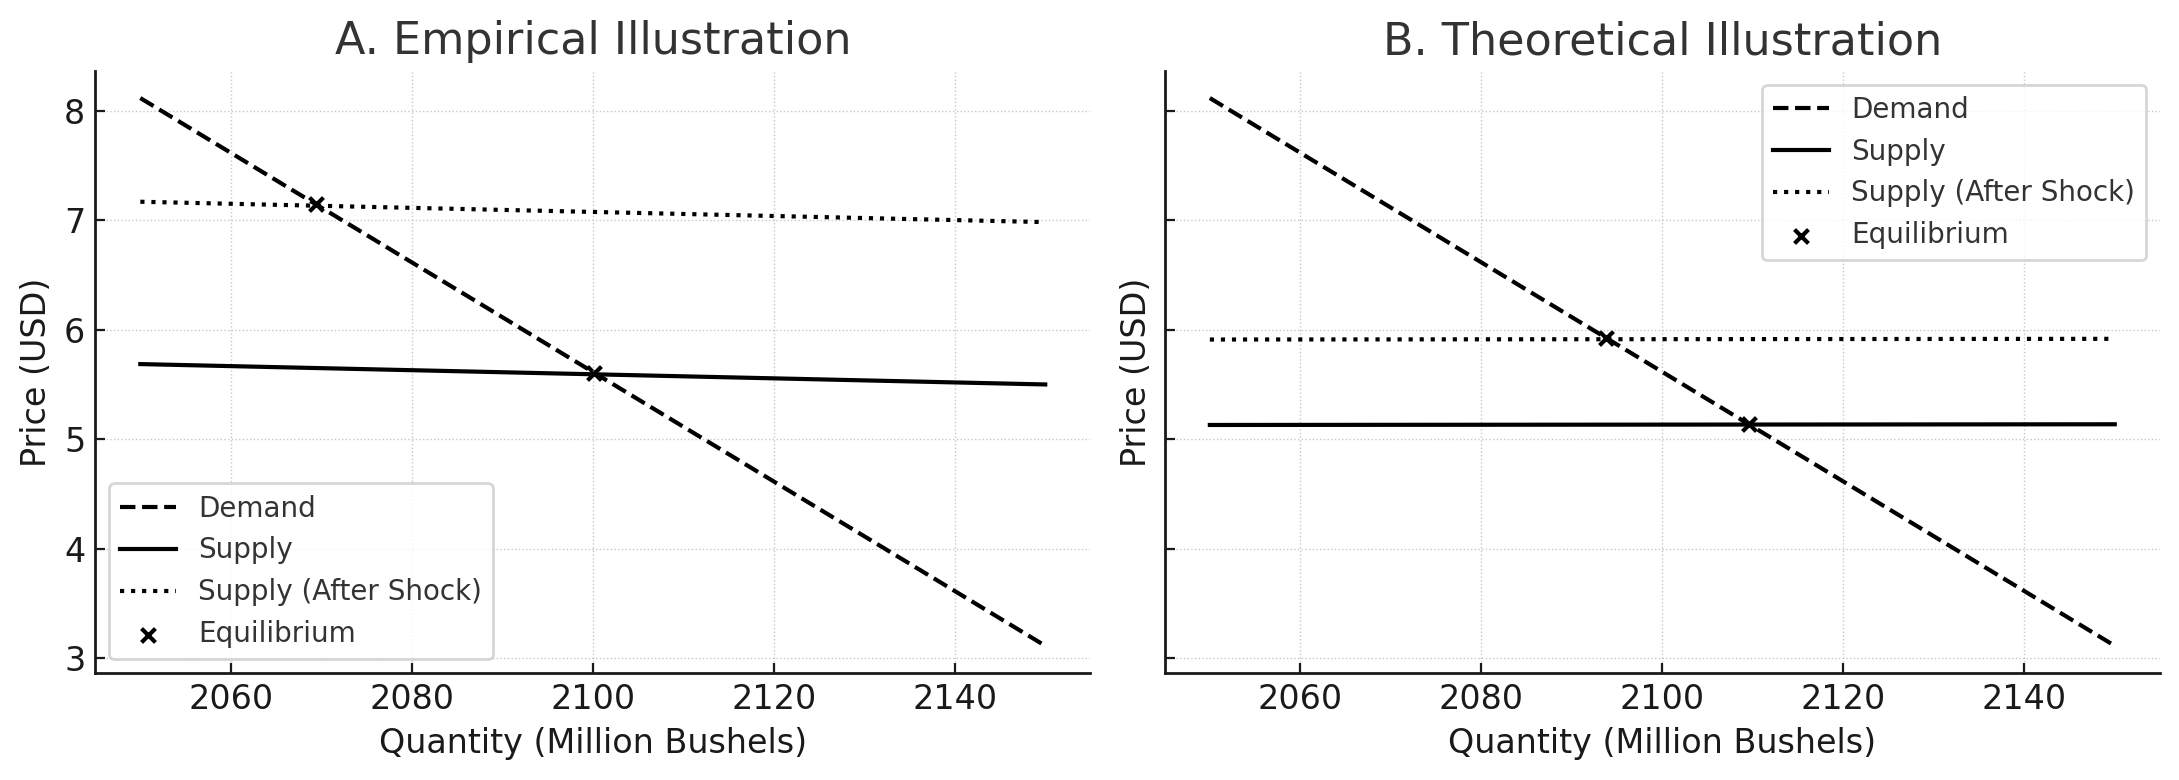
\includegraphics[width=\textwidth]{Hakenes illustration.png}
    \caption{\small{Comparison of empirical and theoretical supply responses to a 15.6\% shock in the U.S. wheat market. Panel A: Empirical supply estimated using OLS. Panel B: Theoretical supply based on the Hakenes–Schliephake (2024) model. Demand is held constant in both cases.}}
\end{figure}


\paragraph{Carbon Footprint Estimation under Empirical Supply Curve:}
To estimate supply behavior, an ordinary least squares (OLS) regression of price is fitted on observed production, yielding the empirical supply curve. In the empirical illustration, the demand curve is specified as linear and downward sloping. Its slope is calibrated using average values from the dataset, consistent with observed market behavior in the U.S. wheat sector. While the curve is not estimated directly via regression (due to data limitations on price responsiveness), it reflects a stylized elasticity based on domain knowledge. This contrasts with the supply curve, which is estimated using OLS on observed price and production data. A supply shock is then simulated for the wheat data in 2016–2017, during which production declined by 15.6\%. 


\paragraph{Carbon Footprint Estimation under Theoretical Supply Curve:}To simulate the same supply shock within the Hakenes and Schliephake (2024) framework, the demand curve from the empirical estimation was retained. However, instead of using a supply curve estimated via ordinary least squares, a theoretically derived supply curve was constructed based on model assumptions. In this approach, firms were assumed to raise capital from households, who in turn optimally allocate their investments under risk. The equilibrium supply curve in this setup is derived from the market-clearing condition and the household's optimal investment response under uncertainty, and takes the form:
\[
P(Q) = c(r_f - \lambda) + \frac{c^2 \alpha \sigma^2}{n - 1} Q,
\]
where the variables retain their definitions as introduced in the derivation. \footnote{See equations 28-36.}

This expression yields a linear and upward-sloping supply curve. The theoretical supply curve applied in this illustration was constructed using parameter values selected to reflect realistic conditions in the U.S. wheat and financial markets during the study period. The marginal cost of production was assumed to be $c = 4$, which is consistent with per-bushel production costs observed in U.S. wheat farming and allows the resulting equilibrium prices to align with historical market levels. The risk-free rate was set to $r_f = 0.05$, corresponding to the average yield on 10-year U.S. Treasury bonds between 2010 and 2016. The liquidation value of capital was taken as $\lambda = 0.01$, reflecting the reduced resale value of farm-specific capital such as machinery or equipment. The coefficient of absolute risk aversion was assumed to be $\alpha = 0.5$, a value that captures moderate household risk sensitivity consistent with empirical estimates from investment literature. The volatility of investment returns was specified as $\sigma = 0.4$, implying a variance of $\sigma^2 = 0.16$, which falls within the range typically observed for U.S. agricultural investments and related financial instruments. Finally, the number of households was assumed to be $n = 100{,}000$, representing an approximation of the number of wheat-producing farms in the United States during the relevant years. These parameter values were used to generate a supply curve that reflects theoretical investment behavior under risk, providing a basis for comparison with the empirically estimated curve, and the intercept reflects the opportunity cost of capital. The new equilibrium values were obtained by solving the intersection of this supply curve with the demand curve used previously.


\subsubsection{Results and Discussion}
In the empirical estimation, the intersection of the two curves provide the empirical equilibrium quantities and prices before and after the 2016–2017 supply shock. This is modeled by proportionally shifting the supply curve upward. Equilibrium price and quantity before and after the shock are obtained by solving the intersection between the demand curve and the respective supply curves and is illustrated in Panel A of Figure 4. The carbon footprint associated with each equilibrium is calculated using an emission factor of 10.88 kg CO\textsubscript{2}e per bushel (based on FAO and USDA estimates) and is presented in Table 6.
\begin{table}[ht]
\captionsetup{justification=raggedright,singlelinecheck=false} 
\caption{Carbon footprint before and after the supply shock using real market data.}
\begin{tabular}{lccc}
\toprule
\textbf{\small{Scenario}} & \textbf{\small{Equilibrium Quantity}} & \textbf{\small{Equilibrium Price}} & \textbf{\small{Carbon Footprint}} \\
\textbf & \small\textbf{(million bushels)} & \small\textbf{(USD)} & \small\textbf{(million kg CO\textsubscript{2}e)} \\
\midrule
\small Before Shock  & \small 2100.71 & \small 5.58 & \small 22859.68 \\
\small After Shock & \small 2068.38 & \small 5.82 & \small 22500.32 \\
\midrule
\small\textbf{Change} & \textemdash& \textemdash& \small\textbf{-359.36} \\
\bottomrule
\end{tabular}
\raggedright
\vspace{0.3cm}

\footnotesize{Source: Author's calculations based on USDA data (2010–2016) and FAO emission factors.}
\end{table}


By solving the intersection of theoretical supply curve with the same demand curve used in the empirical case, equilibrium values for price and quantity were obtained both before and after the simulated shock as shown in Panel B of Figure 4. The corresponding carbon footprints were then computed using the same emissions factor of 10.88 kg CO\textsubscript{2}e per bushel\footnote{See Table 7}.

\begin{table}[ht]
\captionsetup{justification=raggedright,singlelinecheck=false} 
\caption{Model-based carbon footprint before and after the supply shock.}
\begin{tabular}{lccc}
\toprule
\textbf{\small{Scenario}} & \textbf{\small{Equilibrium Quantity}} & \textbf{\small{Equilibrium Price}} & \textbf{\small{Carbon Footprint}} \\
\textbf & \small\textbf{(million bushels)} & \small\textbf{(USD)} & \small\textbf{(million kg CO\textsubscript{2}e)} \\
\midrule
\small Before Shock & \small 2112.45 & \small 5.69 & \small 22983.46 \\
\small After Shock   & \small 2096.36 & \small 5.99 & \small 22808.40 \\
\midrule
\small\textbf{Change} & \textemdash& \textemdash& \small\textbf{-175.06} \\
\bottomrule
\end{tabular}
\raggedright
\vspace{0.3cm}

\footnotesize{Source: Author's calculations based on USDA data (2010–2016) and FAO emission factors.}

\end{table}


\paragraph{Structural Sources of Difference in Emissions Outcomes:}

Although the same demand curve was used in both the empirical and theoretical approaches, the estimated reduction in carbon footprint differed considerably. The empirical estimation yielded a reduction of 359.36 million kg CO\textsubscript{2}e, while the theoretical model predicted a more modest reduction of 175.06 million kg CO\textsubscript{2}e.

This difference can be attributed entirely to the way supply was modeled. In the empirical estimation, the supply curve was estimated via OLS using observed data on price and quantity. This approach captured market behavior as it appeared in the historical record but did not account for underlying decision-making under uncertainty or equilibrium responses. In contrast, the theoretical supply curve was derived from the model’s structural assumptions, incorporating risk preferences, investment volatility, and optimal capital allocation. It reflected how households would respond to market changes under forward-looking behavior, leading to a more muted response in output and, correspondingly, in emissions.

Additionally, the theoretical model introduced a consequentialist perspective by assigning carbon responsibility based on the marginal impact of a household's consumption or investment. In doing so, it internalized substitution effects and capital reallocation, which were not accounted for in the empirical estimation. As a result, while the same emissions formula was applied in both cases, the theoretical model predicted a smaller footprint change due to the buffering effects of equilibrium adjustments. This difference underscores the importance of integrating behavioral dynamics into footprint assessment, particularly when evaluating the impact of shocks or policy interventions.


\section{Responsibility for Household Carbon Emissions}

Households are often portrayed as central actors in climate mitigation—urged to fly less, retrofit their homes, shift their diets, or reduce electricity use. Yet, the basis on which such responsibility is assigned remains contested. What does it mean to hold a household responsible for climate change, and how do we ensure that this responsibility is fair, actionable, and grounded in reality?

Existing carbon accounting methods offer different answers. Some emphasize direct control over emissions, others focus on consumption or supply chains, and still others ask whether a household’s actions actually reduce emissions. These differences reflect deeper questions about agency, influence, and obligation. 

This chapter rethinks household responsibility by comparing the attribution logics embedded in four key models—production-based (GHG Protocol), product-based (LCA), demand-based (EEIO), and marginal impact models (Hakenes and Schliephake). The aim is to evaluate not only how these methods measure emissions, but also how they construct the idea of responsibility itself and with what consequences for policy, fairness, and climate action.

\subsection{Attribution Principles}

\subsubsection{Attribution Based on Operational Control}

Control-based attribution allocates emissions to the actor who directly controls the physical source of greenhouse gas release. Emissions are assigned based on \textit{operational responsibility}, that is, who manages the combustion process or industrial activity rather than on who benefits from or demands the resulting goods and services. In this framework, emissions from electricity generation are attributed to power plants, and those from food or goods production are attributed to manufacturing firms, not to the households that consume the outputs.

The GHG Protocol is the principal framework that operationalizes this logic. In household-level applications, it typically attributes emissions only from direct fuel use (e.g., home heating, personal vehicles) and from purchased electricity or heat (Scopes 1 and 2). Emissions embedded in goods, services, or infrastructure (commonly classified as Scope 3) are excluded unless separately modeled. As a result, household responsibility appears significantly lower than in consumption-based frameworks. For instance, while households in developed economies are responsible for an estimated 60–70\% of emissions under a consumption-based approach, control-based inventories typically attribute only 10–20\% to them.\footnote{See Hertwich and Peters (2009). Consumption-based GHG emissions. \textit{Environmental Science \& Technology}.}

This method reflects a production-based understanding of responsibility: households are held accountable for emissions they physically generate or for energy they purchase, but not for upstream emissions embodied in their consumption. Although narrower in scope, this attribution style serves a clear regulatory function. Its operational clarity makes it particularly suitable for emissions inventories, carbon pricing schemes, and supply-side decarbonization policies that target industrial emitters rather than individuals. The GHG Protocol underpins most national reporting systems and corporate disclosures, and is explicitly aligned with policy instruments such as emissions caps, sectoral mitigation targets, and producer-level carbon accounting.\footnote{See World Resources Institute and WBCSD (2004). \textit{The Greenhouse Gas Protocol: A Corporate Accounting and Reporting Standard}. Also see den Elzen et al. (2020), \textit{Nature Climate Change}, on policy alignment of production-based accounting.} By tracing emissions to producers rather than consumers, control-based attribution enables system-level mitigation efforts without requiring detailed behavioral data at the household level.

\subsubsection{Consumption-Based Attribution}

Consumption-based attribution assigns responsibility for emissions to end users, based on the idea that consumer demand drives production and, ultimately, greenhouse gas emissions. Unlike control-based methods that assign emissions to producers, consumption-based frameworks trace emissions along the supply chain and allocate them to the final household that purchases or uses the good or service.

Among the methods reviewed in this paper, two approaches operationalize consumption-based attribution: life cycle assessment (LCA) and environmentally extended input–output (EEIO) models. Both assign emissions to households for the upstream impacts of their consumption, but they differ in analytical resolution and system boundaries. LCA focuses on product-level analysis by quantifying emissions over a product’s entire life cycle—from raw material extraction through use and disposal.\footnote{Curran, M. A. (2015). Life Cycle Assessment: Principles and Practice. EPA.} This method enables fine-grained comparisons of consumption choices (e.g., meat versus plant-based diets) and supports interventions like eco-labeling and sustainable procurement.

EEIO models, by contrast, estimate emissions based on monetary flows across sectors and are designed to capture systemic effects across entire economies. They link household expenditure data with environmental accounts using national input–output tables, assigning emissions in proportion to spending across categories such as food, transport, and housing.\footnote{Wiedmann, T. (2009). A review of recent multi-region input–output models used for consumption-based emission accounting. \textit{Ecological Economics}.} While LCA relies on detailed process-level data, EEIO models are structured around macroeconomic datasets, making them suitable for national-scale analysis and policy evaluation.

Both approaches consistently attribute a large share of global emissions to households, typically between 60\% and 70\% in high-income countries, by including indirect emissions embedded in consumption.\footnote{Ivanova, D. et al. (2015). Environmental impact assessment of household consumption. \textit{Journal of Industrial Ecology}.} This high attribution has made consumption-based methods influential in shaping narratives around individual climate responsibility and has informed the design of tools such as carbon footprint calculators, dietary guidelines, and voluntary offsetting schemes. However, these methods also risk overstating household agency by abstracting from structural constraints, supply-side inertia, and the availability of low-carbon alternatives.

Despite these limitations, consumption-based attribution provides valuable insights for policymaking. It highlights carbon-intensive lifestyle domains, supports the development of behavioral nudges and fiscal instruments (e.g., carbon taxes or subsidies), and enables differentiated climate strategies across income groups. In this way, it complements production-based models by identifying downstream leverage points for demand-side mitigation.

\subsubsection{Consequentialist Attribution}

The general equilibrium structure and derivation of the Hakenes and Schliephake (2024) model are presented in Chapter~7. Here, we focus specifically on how the model attributes responsibility for emissions—offering a fundamentally different logic from control- or consumption-based methods.

Consequentialist attribution links household responsibility to the actual change in total emissions resulting from marginal economic decisions. In contrast to attribution by operational control or average consumption, this approach estimates how much aggregate emissions would differ if a household were absent from the economy. The household’s carbon footprint is thus defined as the causal marginal impact of its consumption and investment choices on total emissions.

Within the Hakenes–Schliephake framework, emissions are attributed through a counterfactual comparison: the general equilibrium of the full economy versus the equilibrium that would occur if a given household did not participate. Because the model includes both product and financial markets, the resulting footprint incorporates not only direct effects but also indirect spillovers through price mechanisms, risk-adjusted investments, and inter-household substitution. The marginal impact of a household’s behavior is calculated using a weighting parameter, $\phi$, which determines the relative attribution of emissions between consumption and investment.\footnote{Hakenes, H. \& Schliephake, E. (2024). Your Carbon Footprint, Including Investments. SSRN 4710536. See also Section~7.1.4 in this thesis for derivation of $\phi$.}

This weighting is sensitive to structural characteristics of the economy: greater risk aversion or financial volatility shifts responsibility toward consumption, while higher substitutability across sectors amplifies the spillover effect through investment. As a result, households are only held responsible for emissions they can meaningfully influence. If consumption is perfectly substitutable or investment flows are fully absorbed by other agents, the attributed footprint may approach zero—even if the household’s nominal expenditure is large.

By assigning responsibility based on marginal system-wide impact, the model avoids double-counting and mitigates the over-attribution seen in static frameworks. It also aligns well with policy approaches that emphasize structural levers, such as green financial regulation or carbon-intensity weighting of investment portfolios. While less intuitive and more data-intensive than other methods, this attribution logic provides a refined lens for distinguishing symbolic from substantive household climate action.

\subsection{Comparative Analysis of Attribution Principles}

Attribution methods differ not only in analytical structure but in how they frame responsibility—what they assign to households, what they assume about agency, and what they ignore. As visualized in Figure~\ref{fig:heatmap}, these differences create meaningful trade-offs that shape both interpretation and policy relevance.

Control-based attribution (GHG Protocol) limits household responsibility to direct actions, minimizing the risk of over-attribution but offering little behavioral or structural insight. Consumption based approaches (LCA and EEIO) invert this: they assign large shares of emissions to households, enabling lifestyle-oriented analysis but often abstracting from real-world constraints, rebound effects, or structural inertia. They perform well descriptively but struggle to differentiate between symbolic and effective action.

Only the Hakenes and Schliephake model formally incorporates systemic feedbacks. Its consequentialist logic reframes attribution as marginal influence, not average burden. This avoids double-counting and grounds responsibility in causal agency, but at the cost of complexity, abstraction, and limited communicability.
\begin{figure}[h]
    \centering
    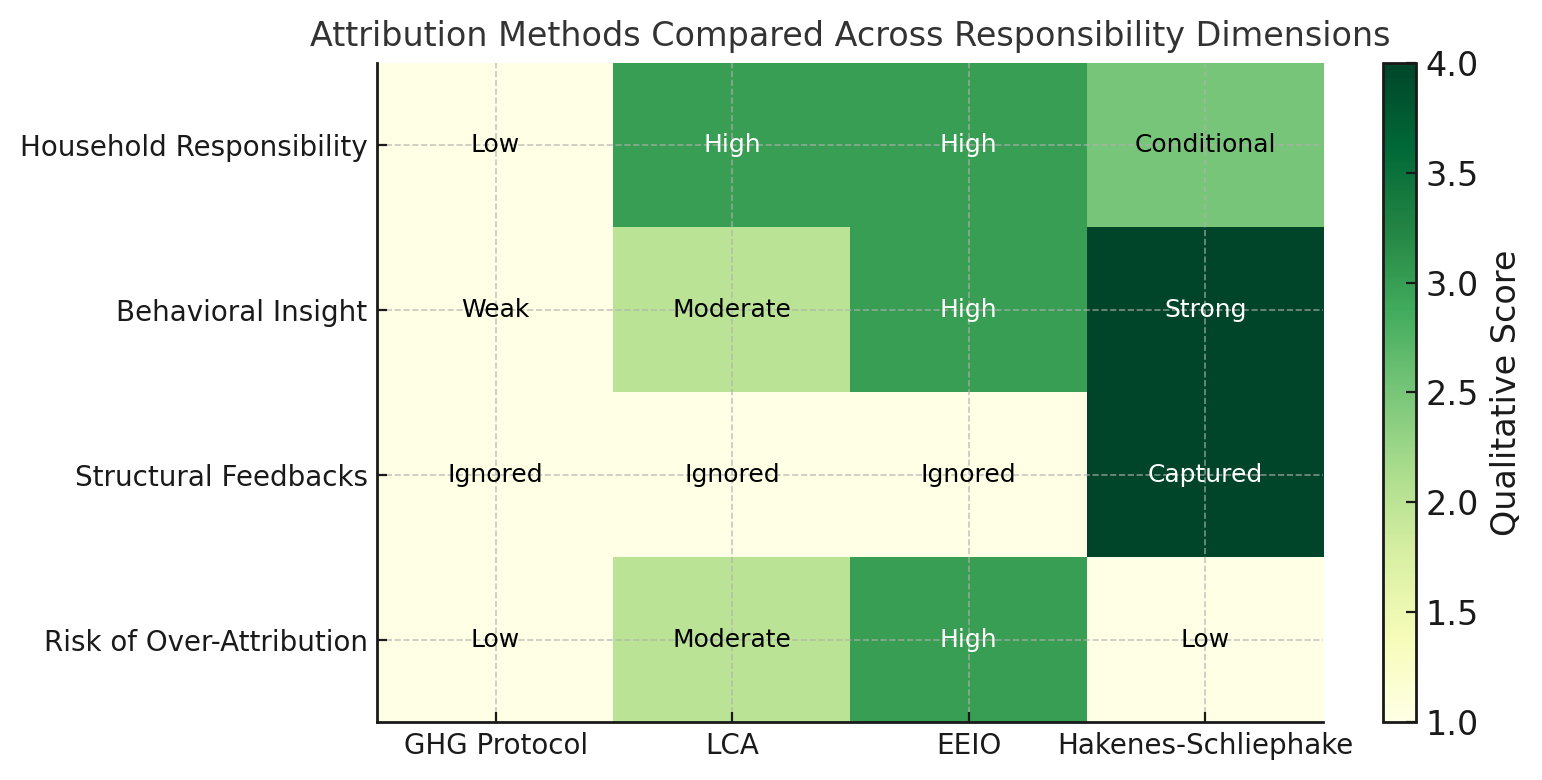
\includegraphics[width=0.8\textwidth]{Heatmap Res.png}
    \caption{\small{Comparative heatmap of attribution frameworks across key responsibility dimensions. Higher scores indicate greater behavioral relevance, structural sensitivity, or risk of over-attribution. Source: Author's own analysis based on Hertwich and Peters (2009), Ivanova et al. (2015), Hakenes and Schliephake (2024), and Capstick et al. (2021).}}\label{fig:heatmap}
\end{figure}
Figure~\ref{fig:heatmap} illustrates this spectrum: methods differ in how much they reveal about behavioral influence, how they treat economic structure, and how carefully they delimit the scope of household responsibility. Choosing an attribution framework is therefore not just a technical exercise—it reflects underlying assumptions about fairness, tractability, and what forms of action are worth encouraging.



\noindent
The discussion establishes a basis for the following chapter, which examines how different attribution logics align with climate policy instruments and what this implies for equitable mitigation strategies.
\section{Policy Instruments for Household Decarbonization}

As climate policy increasingly turns its attention to households, a critical insight emerges: household emissions are neither uniform nor equally reducible. Per capita emissions vary significantly across regions. In the European Union, for example, households in Eastern Europe tend to emit less, while countries like France and Norway benefit from cleaner electricity, resulting in lower emissions despite comparable consumption levels (see Figure 6).
\begin{figure}[h]
    \centering
    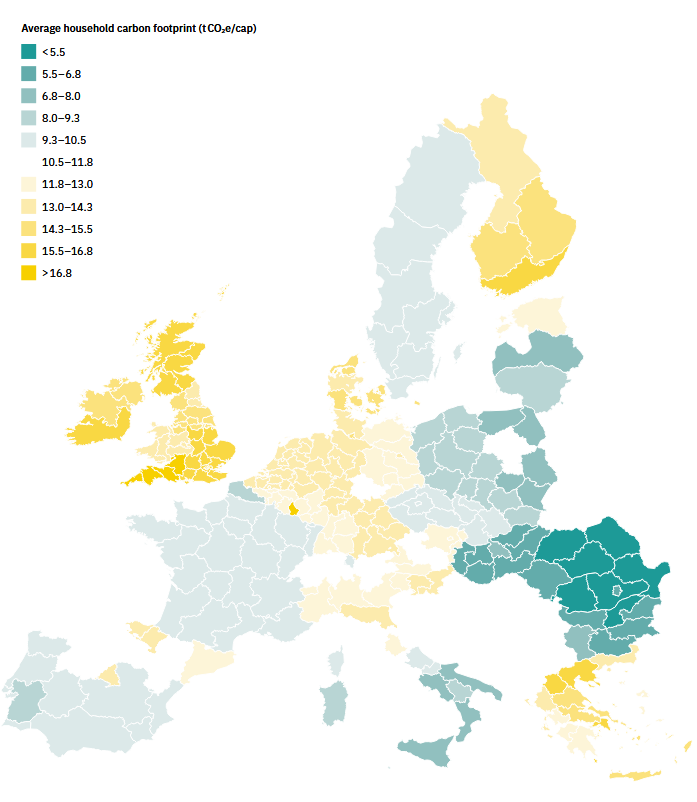
\includegraphics[width=0.7\textwidth]{per capita world emissions.png}
    \caption{\small{Average household carbon footprint in Europe (t CO$_2$e/cap) (Source: Ivanova et al., 2017)}}\label{fig:percapita}
\end{figure}

Layered onto these geographic disparities are stark inequalities across income groups. Globally, the wealthiest 10\% are responsible for nearly half of lifestyle-related emissions, while the poorest 50\% account for just 10\% (Figure 7). These imbalances not only challenge the adequacy of uniform policy tools but also raise broader concerns about fairness, capacity, and the political viability of climate action.

\begin{figure}[h]
    \centering
    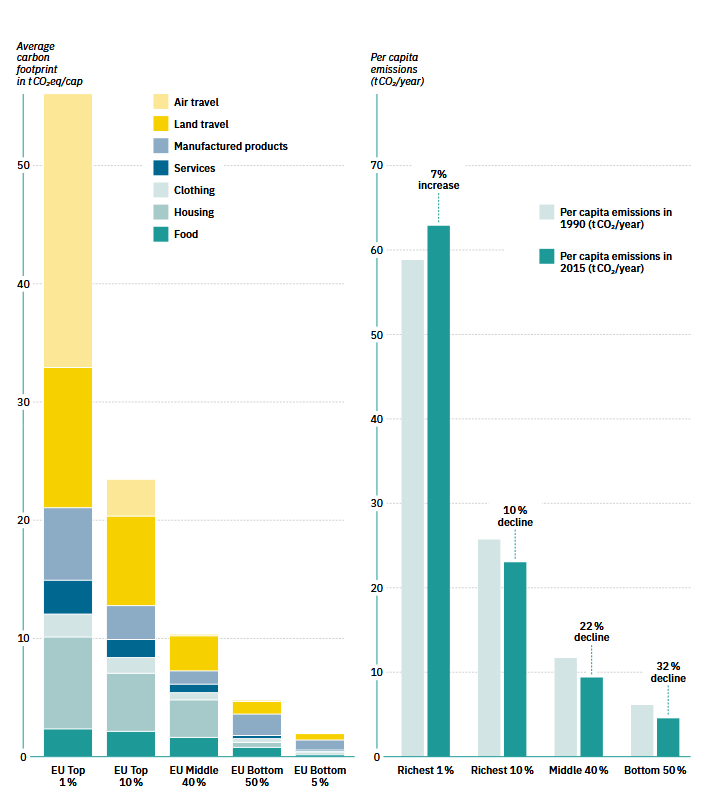
\includegraphics[width=0.8\textwidth]{emission by income.png}
    \caption{\small{(Left) Average carbon footprint (CF) distribution by consumption category in the European Union (Ivanova et al., 2017). (Right) Per capita consumption emissions (t CO$_2$/year) by EU income group in 1990 and 2015 (Gore \& Alestig, 2020)}}
\end{figure}

This chapter shifts focus from identifying \textit{who} is responsible for emissions, as discussed previously, to examining \textit{how} that responsibility is translated into policy. It explores the relationship between carbon accounting methods and the instruments they inform. Whether a policy targets energy use, product design, financial portfolios, or consumption behavior depends largely on the accounting framework through which household emissions are assessed.

Each method—the GHG Protocol, LCA, EEIO, and the Hakenes-Schliephake model—rests on distinct assumptions about agency, boundaries, and causality, which shape policy design. The GHG Protocol informs direct emission controls; LCA supports product-level regulation; EEIO enables upstream, consumption-based interventions; and equilibrium models capture behavioral and financial spillovers. This chapter maps core instruments—carbon taxes, product and appliance standards, investment-based instruments, behavioral interventions, and AI based digital tools—to their methodological bases, assessing their mitigation potential and distributive impact.

\subsection{Carbon Taxes}

Carbon taxation remains one of the most established and economically coherent instruments for reducing greenhouse gas emissions. Implemented in over 30 jurisdictions, tax rates range widely---from under 5~USD per tonne of CO\textsubscript{2} in countries such as South Africa and Argentina to over 130~USD in Sweden, where sustained taxation has contributed to a 27\% reduction in territorial emissions since 1990 alongside continued economic growth. These taxes are typically grounded in the GHG Protocol, targeting direct (Scope~1) and energy-related (Scope~2) emissions. As such, they primarily influence household-level consumption of motor fuels, heating, and electricity.

However, this production-based accounting framework captures only a portion of household carbon footprints, particularly in high-income economies where a significant share of emissions is embodied in imported goods. To address this limitation, Environmentally Extended Input-Output (EEIO) models offer a broader perspective by tracing emissions along global supply chains. EEIO-based extensions to carbon tax design enable the implementation of \textit{consumption-based taxation}, targeting emissions embedded in products such as food, electronics, and apparel---regardless of origin. This analytical foundation supports emerging instruments such as \textit{Border Carbon Adjustments} (BCAs), which impose equivalent carbon prices on imports to prevent leakage and align international trade with domestic climate objectives.

Equity considerations remain central to the legitimacy of carbon taxation. Standard carbon taxes tend to be regressive, disproportionately affecting lower-income households that allocate a greater share of expenditure to energy and basic goods. EEIO-informed approaches offer more differentiated insight into household consumption profiles, allowing for progressive compensation mechanisms, product-specific exemptions, or redistributive revenue recycling schemes. Ultimately, the effectiveness and fairness of carbon taxation depend not only on price levels, but on the accounting principles underpinning their design and the socio-economic context into which they are embedded.


\subsection{Product and Appliance Standards}

Product and appliance standards are among the most established policy instruments for reducing household emissions. Grounded in Life Cycle Assessment (LCA), they address carbon impacts across a product’s entire lifespan—production, use, and disposal—allowing regulators to set minimum energy performance and environmental criteria that reflect full emissions intensity rather than just operational use.

The European Union’s Ecodesign Directive, first introduced in 2009, exemplifies this approach. It has been credited with saving over 230 million tonnes of CO\textsubscript{2} equivalent annually by progressively eliminating inefficient appliances from the market. Its latest extension—the 2022 proposal for the Ecodesign for Sustainable Products Regulation (ESPR), adopted in 2023—broadens the framework to include embedded carbon, durability, reparability, and circularity requirements across nearly all physical goods placed on the EU market. The synergetic effect of Ecodesign and energy labelling policies is illustrated in Figure~\ref{fig:ecodesign}.

\begin{figure}[htbp]
  \centering
  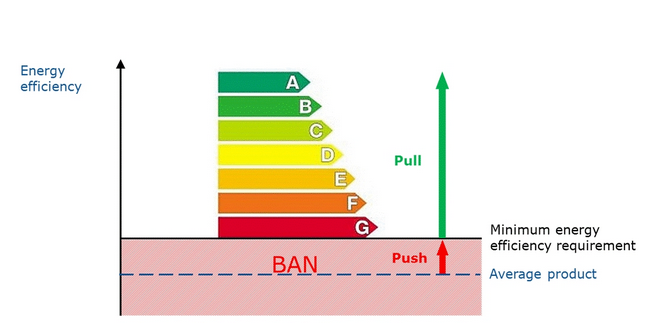
\includegraphics[width=0.6\textwidth]{ecodesign.png}
  \caption{\small{Synergetic effects of Ecodesign and Energy Labelling in the EU. Source: European Commission (2023)}}\label{fig:ecodesign}
\end{figure}

Internationally, similar policies have been adopted through Japan’s Top Runner Program and the United States’ appliance efficiency rules under the Energy Policy and Conservation Act and California Consumer Protection Act (CCPA). At COP26, the Product Efficiency Call to Action (2021) brought together over 20 countries to commit to higher minimum efficiency standards for four key product categories. Beyond appliances, the EU has also introduced product-level restrictions for high-carbon industrial inputs, such as steel and aluminium, based on lifecycle emissions thresholds.

While highly effective in formal markets, the broader success of product standards depends on enforcement capacity, affordability of compliant goods, and access to clean technologies. Without complementary measures such as subsidies or inclusive design, these policies risk excluding lower-income households. Greenwood and Warren (2022) highlight that energy-efficient technologies are often underutilized in low-income settings due to symbolic preferences, limited affordability, and mismatched design priorities. As such, standards without adequate behavioral and financial support can reinforce inequality or lead to parallel use of inefficient alternatives. Nevertheless, LCA-based product standards remain a cornerstone of household and supply-chain decarbonization strategies, particularly when integrated into broader circular economy and trade frameworks.

\subsection{Investment-Based Instruments}
An increasing share of global emissions can be traced not to direct consumption, but to the investment behavior of affluent households. As wealth concentration rises, so too does the influence of household portfolios on the financing of emissions-intensive sectors. Investment-based climate instruments seek to reallocate capital toward low-carbon assets by incorporating emissions responsibility into financial decision-making frameworks.

A theoretical perspective on this dynamic is offered by the general equilibrium model developed by Hakenes and Schliephake (2024), which frames households as both consumers and investors. In this setup, portfolio decisions are shaped by risk preferences, capital endowments, and cross-sectoral spillovers and serve as indirect channels through which households influence aggregate emissions. Emissions responsibility, accordingly, is not limited to final demand but extends to patterns of asset ownership and capital allocation and can be complemented by EEIO data to parameterize sectoral emission intensities and inter-industry linkages.

Policy mechanisms informed by this logic include cap-and-trade systems such as the EU Emissions Trading System (EU ETS), California Carbon Allowance program, and the Regional Greenhouse Gas Initiative (RGGI). These platforms internalize carbon costs into financial assets via tradable permits, altering the relative returns of high- versus low-emission sectors. Compliance and voluntary carbon markets (CCM and VCM) complement these by commodifying offsets and channeling investment into renewables, afforestation, and carbon removal.

Building on these policy mechanisms, financial markets have introduced instruments that embed climate risk and incentivize sustainability alignment. These include green and sustainability-linked bonds (SLBs), ESG-focused ETFs \footnote{Environmental, Social, and Governance (ESG) Exchange-traded funds (ETFs) track portfolios screened for the ESG criteria}, and carbon derivatives. For instance, the EU Green Bond Standard and rising carbon futures prices under the EU ETS make compliant, low-emission investments more financially attractive.

From a distributional perspective, investment-based instruments offer a corrective to the narrow focus of traditional consumption-side policy. Empirical studies show that the top 10\% of households in the United States account for over 40\% of national emissions, largely through capital income and asset ownership. The top 1\% alone is responsible for approximately 17\%. Instruments that tax fuel or regulate appliances have limited reach in this demographic. By contrast, integrating emissions accountability into investment performance metrics, fiduciary standards, and capital gains taxation offers a scalable mechanism to shift the carbon profile of global capital markets.

However, the political feasibility of these instruments remains constrained by data limitations, regulatory asymmetries, and the entrenched power of asset holders. Their long-term success depends not only on market design and disclosure standards, but also on embedding equity concerns into financial governance---ensuring that decarbonization does not exacerbate wealth disparities, but rather aligns emissions responsibility with financial capacity.


\subsection{Behavioural Interventions}

Behavioral interventions target the psychological, social, and cultural dimensions of household emissions, complementing price and technology-based approaches. These strategies aim to shift routines such as mobility, cooking, or appliance use through nudges, symbolic cues, default settings, and co-design. They are typically evaluated via randomized trials, adaptive field experiments, and pilot programs tracking real-time behavioral change.

Khanna et al.\ (2021) find that monetary incentives reduce energy use by 12--20\%, while non-monetary nudges average 7--12\%. At scale, such interventions could mitigate up to 0.35~GtCO\textsubscript{2} annually. Marchi et al.\ (2021) estimate that targeted behavioral changes in diet, mobility, housing, and appliances can lower household footprints by up to 25\%, with high-impact actions reducing emissions by 1.5--2.5~tCO\textsubscript{2}e per capita each year\footnote{ A detailed version of behaviourial change and their expected outcome on carbon footprint appears in Table A10 of Appendix A.}.

In this context, the relevance of carbon accounting methods becomes clear. Traditional frameworks like the GHG Protocol and LCA assume fixed usage patterns and stable preferences, making them poorly suited to capture behavioral fluidity. Even EEIO models typically aggregate consumer behavior into average sectoral flows, rendering behavioral heterogeneity invisible. As a result, these models underestimate the mitigation potential of behavioral instruments and are rarely used to design or evaluate them. The general equilibrium model by Hakenes and Schliephake offers a partial corrective by incorporating household preferences and spillovers in a dynamic system. While primarily focused on investment behavior, the model’s structure could be adapted to simulate preference shifts and their economy-wide effects over time. 

To be effective, however, behavioral interventions must be embedded in broader systems. Khanna et al. (2021) stress the need for institutional integration, and Greenwood and Warren (2022) highlight the failure of top-down programs that ignore cultural context—as seen in cookstove initiatives abandoned due to gender norms or culinary practices. Especially in low-income settings, behavioral tools offer high-trust, low-cost mitigation, if supported by adaptive policies that account for persistence, equity, and social context. Without such integration, they risk being sidelined by the very models that shape climate governance.
\subsection{AI enabled Digital Platforms}

Artificial intelligence (AI) and digital platforms are reshaping how household emissions are measured, communicated, and influenced. Their core methodological advantage lies in processing high-dimensional, heterogeneous data across spending, energy use, location, and behavior. Machine learning models can estimate emissions at the transaction level, outperforming EEIO models in granularity, and adapting to behavioral change more dynamically than static LCA approaches.

Practical implementations are already emerging. The Swedish app \textit{Svalna} uses financial data to estimate emissions and recommend reductions, while \textit{Klima} simulates behavioral shifts and offset strategies. Smart meters in countries like the UK and France integrate with nudging platforms that use reinforcement learning to reduce household energy demand. AI is also entering personal finance tools to automate carbon accounting for investment portfolios, aligning with investment-based attribution frameworks such as Hakenes--Schliephake.

A representative example is Moneythor’s carbon tracking engine, which links banking transactions to emissions data using EEIO-derived factors. Each purchase is categorized and assigned a CO\textsubscript{2} weight, producing real-time feedback dashboards and behavioral nudges. This form of embedded carbon accounting enhances precision and responsiveness while integrating smoothly with financial decision-making platforms. Figure~\ref{fig:carbontracker} illustrates how such systems enable users to monitor their carbon impact through digital banking interfaces.

\begin{figure}[htbp]
\centering
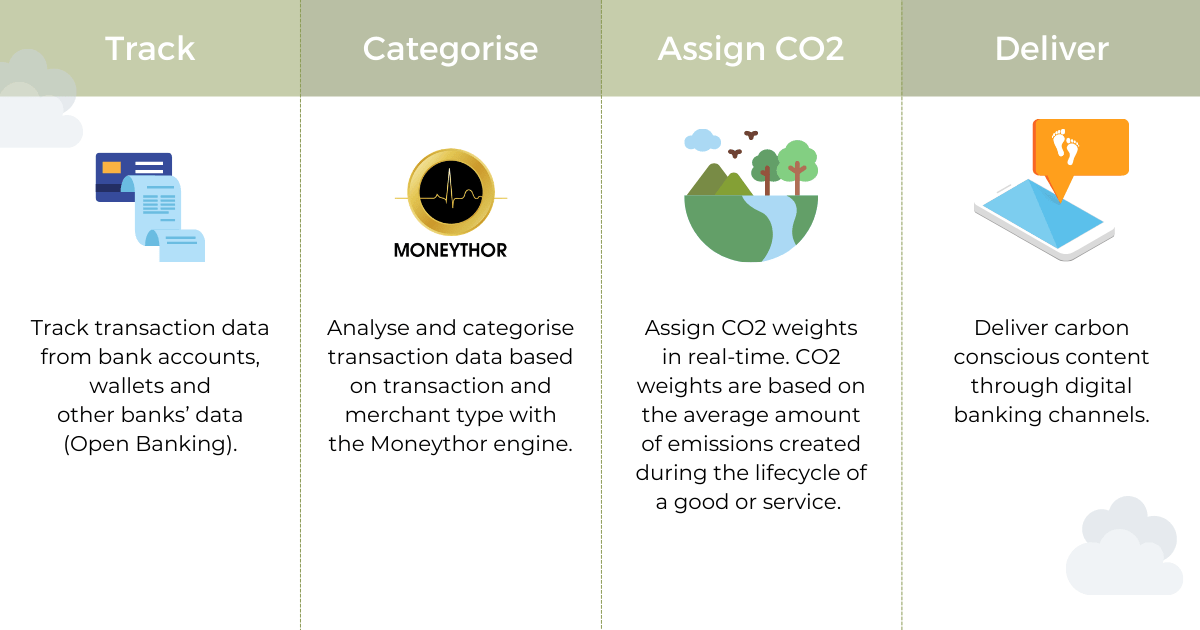
\includegraphics[width=0.8\textwidth]{moneythor.png} % Replace with actual file name
\caption{\small{Illustration of AI-enabled household carbon tracking via transaction-level banking data. Tools like Moneythor categorize spending, apply EEIO-based emissions factors, and deliver personalized dashboards. Source: Moneythor (2021)}}
\label{fig:carbontracker}
\end{figure}

Climate finance institutions are beginning to support digital infrastructure such as open emissions APIs, interoperable energy data hubs, and identity-linked carbon registries. These investments can enable adaptive policy targeting, but must be designed with digital equity in mind. As Greenwood and Warren (2022) caution, in low-income or rural contexts where smartphone and broadband access are limited, digital tools risk deepening exclusion rather than empowering mitigation.

Governance challenges persist. Algorithmic opacity and commercial control of emissions data raise concerns about consent, accuracy, and accountability. Without robust standards, digital sustainability platforms may incentivize superficial compliance while deflecting attention from structural emissions drivers. Moreover, overreliance on individual responsibility narratives can obscure the systemic dimensions of household emissions.

Nonetheless, when embedded within participatory design frameworks, open standards, and inclusive digital finance, AI tools can significantly extend the reach and adaptability of household carbon policy. They enable households not only to monitor emissions, but to co-create mitigation pathways grounded in data, context, and agency.

\subsection{Comparative Analysis of Policy Instruments}

Effective household decarbonization requires a policy toolkit that aligns with both attribution methodologies and systemic drivers of emissions. The five household-level policy instruments examined in this chapter—carbon taxes, product standards, investment-based tools, behavioral interventions, and AI-enabled platforms—emerge from distinct methodological traditions and reflect different logics of carbon attribution. Their alignment with accounting frameworks such as the GHG Protocol, Life Cycle Assessment (LCA), Environmentally Extended Input-Output (EEIO) analysis, and the general equilibrium model of Hakenes and Schliephake determines not only how emissions are measured, but how responsibility is assigned and policies are justified.

Each attribution method presents both analytical strengths and inherent limitations. The GHG Protocol provides regulatory clarity and institutional standardization, but focuses narrowly on direct emissions, overlooking behavioral dynamics and financial externalities. LCA enables detailed product-level assessments and supports eco-design, yet it struggles with system boundaries and typically excludes indirect effects beyond the supply chain. EEIO expands accountability to upstream and imported emissions, offering systemic coverage, but requires harmonized data and lacks granularity at the household level. General equilibrium models capture financial flows, substitution effects, and inequality, but are computationally intensive and sensitive to model assumptions. Behavioral science and AI facilitate individualized, adaptive interventions with real-time feedback, though they lack formal integration into existing carbon accounting and financing architectures. These methodological trade-offs determine how emissions are quantified, responsibility is assigned, and which instruments are most effectively deployed (see Table 8)
\begin{table}[h]
\centering
\caption{Household Carbon Policy Instruments: Methodological Alignment and Strategic Implications}
\label{tab:final_policy_comparison}
\begin{threeparttable}
\resizebox{\textwidth}{!}{%
\begin{tabular}{L{3.8cm} L{4.2cm} L{3.3cm} L{3.8cm} L{4cm}}
\toprule
\textbf{Policy Instrument} & \textbf{Methodological Basis} & \textbf{Climate Finance Compatibility} & \textbf{Strengths} & \textbf{Limitations} \\
\midrule
Carbon Taxes & GHG Protocol (Scope 1–2); extended by EEIO for consumption-based pricing & Moderate\tnote{1} & Transparent, administratively simple; scalable across sectors & Regressive without redistribution; ineffective without embedded emissions accounting \\
\addlinespace
Product and Appliance Standards & Life Cycle Assessment (LCA); partially supported by GHG Protocol & High\tnote{2} & Technologically mature; harmonized with global trade and procurement policies & Poor alignment with cultural practice; limited uptake in informal settings \\
\addlinespace
Investment-Based Instruments & General Equilibrium (Hakenes–Schliephake), supported by EEIO & Moderate\tnote{3} & Targets systemic inequality and capital-linked emissions; long-term structural potential & Requires fiscal system reform; politically sensitive in high-income contexts \\
\addlinespace
Behavioral Interventions & Behavioral science; weakly embedded in traditional carbon models & High\tnote{4} & Low-cost, participatory, socially adaptive; crucial in informal or transitional settings & Difficult to quantify and fund through conventional carbon metrics; often undervalued \\
\addlinespace
AI enabled Digital Platforms & Hybrid: EEIO + LCA + behavioral integration & Growing\tnote{5} & Enables real-time, household-specific carbon tracking; bridges data with policy simulation & Digital exclusion risks; regulatory and privacy concerns in implementation \\
\bottomrule
\end{tabular}
}
\raggedright
\footnotesize\textit{Notes:}
\begin{tablenotes}
\footnotesize
\item[1] Adopted in Sweden, Canada, and Chile; climate finance relevance via carbon dividends and fiscal transition funding.
\item[2] Supported by GCF, bilateral donors, and national public procurement standards (e.g., EU Ecodesign Directive).
\item[3] Potential integration into sovereign wealth funds, IMF tax proposals, and fiduciary regulation.
\item[4] Increasingly funded via GEF and UNDP behavioral pilots, especially where co-benefits (e.g., health, gender) apply.
\item[5] Enabled through blended finance, fintech partnerships, and smart city infrastructure initiatives.
\end{tablenotes}
\end{threeparttable}
\end{table}

\subsection{Policy Recommendations}

The analysis shows that household carbon footprint estimates and the policy narratives they support depend fundamentally on the chosen attribution method. In light of these findings, it is recommended that policymakers adopt a layered approach to household decarbonization, combining complementary instruments rather than relying on a single metric or intervention. 

Policymakers should expand the use of carbon pricing to include both direct and indirect household emissions. While traditional carbon taxes remain important for regulating direct fuel and electricity use (as captured by the GHG Protocol), they should be complemented by upstream pricing mechanisms that reflect embedded emissions in imported goods and services. This could take the form of border carbon adjustments or sector-level pricing tied to EEIO-based emission intensities.

Financial regulators should begin attributing emissions from capital markets back to households through investment-linked accounting. This includes the integration of carbon intensity metrics into retail investment products, mandatory reporting of household investment footprints by financial institutions, and exploration of capital gains tax differentials based on portfolio emissions. These measures are directly supported by the attribution logic of the Hakenes-Schliephake model, which links household investment to market-wide externalities.

To shift household behavior more effectively, governments should invest in digital tools that provide individualized, real-time carbon feedback. Specifically, it is recommended that national climate agencies partner with fintech and data providers to develop open-source, AI-enabled carbon tracking apps tied to bank transactions, utility data, and purchasing patterns. These tools should be integrated into existing incentive programs, such as green vouchers, eco-bonuses, or climate income schemes, to reward emissions reductions at the household level.

Product regulation should be strengthened in high-emission consumption categories such as housing, transport, and food. LCA and EEIO-based models show that material-intensive and frequently used goods contribute disproportionately to household footprints. It is therefore recommended that EU Ecodesign standards and national efficiency labels be extended to include embodied carbon and lifetime emissions, and that carbon-based criteria be added to public procurement and product labelling systems.

Finally, future research should focus on building hybrid empirical models that integrate household consumption, investment, and behavioral data. This includes dynamic extensions of the Hakenes-Schliephake model, disaggregated EEIO applications using household microdata, and behavioral segmentation in carbon tracking platforms. Special attention should be given to developing policy simulations that can account for differential impacts across income groups, asset ownership, and urban-rural contexts.

\section{Conclusion}

This thesis examined the implications of methodological choice in estimating household carbon footprints and its consequences for climate policy design. Through a comparative analysis of four established approaches—the GHG Protocol, Life Cycle Assessment (LCA), Environmentally Extended Input-Output (EEIO) analysis, and the general equilibrium model of Hakenes and Schliephake, the study highlighted the variation in footprint outcomes and their sensitivity to attribution frameworks.

The empirical illustrations suggest carbon estimates diverge substantially across methods. Process-based and direct accounting techniques (GHG Protocol, LCA) tend to generate lower household-level footprints, as they limit responsibility to immediate consumption and energy use. In contrast, EEIO and equilibrium models yield significantly higher values by incorporating supply chain externalities, inter-industry linkages, and financial market effects. As a result, method choice affects not only the scope and magnitude of household footprint estimates but also the visibility of household contributions to aggregate carbon emissions.

Consequently, each method supports a distinct set of policy instruments. The GHG Protocol provides a suitable basis for implementing direct fuel taxation and energy pricing; LCA supports appliance standards and eco-design regulation; EEIO estimates support policies targeting upstream emissions, such as import carbon adjustments, and the general equilibrium model provides the analytical basis for investment-based taxation and capital-sensitive interventions. These methodological linkages are critical to ensuring internal consistency between carbon accounting, policy targeting, and financing strategy.


The study has several limitations. It relies on the use of stylized data in the empirical illustration, the static formulation of the equilibrium model, and the absence of behavioral heterogeneity and temporal dynamics. Future work should incorporate micro-level household datasets, extend the equilibrium approach to simulate intertemporal feedbacks, and explore the integration of behavioral and digital mechanisms into accounting models and policy evaluation.

Overall, the findings underscore that the design of household carbon policy cannot be separated from methodological decisions. Attribution frameworks shape the scale, focus, and fairness of climate interventions. A methodologically coherent and policy-aligned approach is essential for building effective, equitable, and finance-compatible decarbonization strategies at the household level.

\newpage

\section*{References}
\addcontentsline{toc}{section}{References}



\vspace{0.5em}
{\small
\noindent
\parbox{\linewidth}{
\hangindent=1.5em
\hangafter=1
Baiocchi, G., Minx, J., \& Hubacek, K. (2010). The impact of social factors and consumer behavior on carbon dioxide emissions in the United Kingdom. \textit{Journal of Industrial Ecology}, 14(1), 50–72. \\
DOI: \href{https://doi.org/10.1111/j.1530-9290.2009.00216.x}{10.1111/j.1530-9290.2009.00216.x}
}
}

{\small
\noindent
\parbox{\linewidth}{
\hangindent=1.5em
\hangafter=1
Crawford, R. H., Bontinck, P.-A., Stephan, A., Wiedmann, T., \& Yu, M. (2018). Hybrid life cycle inventory methods – A review. \textit{Journal of Cleaner Production}, 172, 1273–1288. \\
DOI: \href{https://doi.org/10.1016/j.jclepro.2017.10.176}{10.1016/j.jclepro.2017.10.176}
}
}

\vspace{0.5em}
{\small
\noindent
\parbox{\linewidth}{
\hangindent=1.5em
\hangafter=1
Cabernard, L., Pfister, S., Oberschelp, C., \& Hellweg, S. (2022). Growing environmental footprint of plastics driven by coal combustion. \textit{Nature Sustainability}, 5(2), 139–148. \\
DOI: \href{https://doi.org/10.1038/s41893-021-00807-2}{10.1038/s41893-021-00807-2}
}
}

\vspace{0.5em}
{\small
\noindent
\parbox{\linewidth}{
\hangindent=1.5em
\hangafter=1
Capstick, S., Khosla, R., \& Wang, S. (2021, January 21). \textit{Bridging the gap – the role of equitable low-carbon lifestyles}. UN Environment Programme. \\
Available at: \href{https://www.un-ilibrary.org/content/books/9789280738124c010}{un-ilibrary.org/content/books/9789280738124c010}
}
}

\vspace{0.5em}
{\small
\noindent
\parbox{\linewidth}{
\hangindent=1.5em
\hangafter=1
Curran, M. A. (2015). \textit{Life Cycle Assessment Student Handbook}. Wiley, Hoboken, 320 p. \\
Available at: \href{https://www.scirp.org/reference/referencespapers?referenceid=2765754}{scirp.org/referenceid=2765754}
}
}

\vspace{0.5em}
{\small
\noindent
\parbox{\linewidth}{
\hangindent=1.5em
\hangafter=1
Jackson, A., Druckman, A., \& Jackson, T. (2024). The carbon footprint of UK households 1990–2004: A socio-economically disaggregated, quasi-multi-regional input–output model. \textit{Ecological Economics}, 68(7), 2066–2077. \\
Available at: \href{https://econpapers.repec.org/article/eeeecolec/v_3a68_3ay_3a2009_3ai_3a7_3ap_3a2066-2077.htm}{econpapers.repec.org/...}
}
}

\vspace{0.5em}
{\small
\noindent
\parbox{\linewidth}{
\hangindent=1.5em
\hangafter=1
Dubois, G., Sovacool, B., Aall, C., Nilsson, M., Barbier, C., Herrmann, A., Bruyère, S., Andersson, C., Skold, B., Nadaud, F., Dorner, F., Moberg, K. R., Ceron, J. P., Fischer, H., Amelung, D., Baltruszewicz, M., Fischer, J., Benevise, F., Louis, V. R., \& Sauerborn, R. (2019). It starts at home? Climate policies targeting household consumption and behavioral decisions are key to low-carbon futures. \textit{Energy Research \& Social Science}, 52, 144–158. \\
DOI: \href{https://doi.org/10.1016/j.erss.2019.02.001}{10.1016/j.erss.2019.02.001}
}
}

\vspace{0.5em}
{\small
\noindent
\parbox{\linewidth}{
\hangindent=1.5em
\hangafter=1
European Commission. (2024). \textit{Ecodesign for Sustainable Products Regulation}. European Commission. \\
Available at: \href{https://commission.europa.eu/energy-climate-change-environment/standards-tools-and-labels/products-labelling-rules-and-requirements/ecodesign-sustainable-products-regulation_en}{commission.europa.eu/...}
}
}

\vspace{0.5em}
{\small
\noindent
\parbox{\linewidth}{
\hangindent=1.5em
\hangafter=1
Gore, T., \& Alestig, M. (2020). \textit{Confronting Carbon Inequality in the European Union: Why the European Green Deal Must Tackle Inequality While Cutting Emissions}. Oxfam Media Briefing.
}
}

\vspace{0.5em}
{\small
\noindent
\parbox{\linewidth}{
\hangindent=1.5em
\hangafter=1
Greenwood, N., \& Warren, P. (2022). Climate risk disclosure and climate risk management in UK asset managers. \textit{International Journal of Climate Change Strategies and Management}, 14, 272–292. \\
Available at: \href{https://www.scirp.org/reference/referencespapers?referenceid=3699092}{scirp.org/referenceid=3699092}
}
}

\vspace{0.5em}
{\small
\noindent
\parbox{\linewidth}{
\hangindent=1.5em
\hangafter=1
Guinée, J. B., \& Heijungs, R. (2011). Life cycle sustainability analysis. \textit{Journal of Industrial Ecology}, 15(5), 656–658. \\
DOI: \href{https://doi.org/10.1111/j.1530-9290.2011.00398.x}{10.1111/j.1530-9290.2011.00398.x}
}
}

\vspace{0.5em}
{\small
\noindent
\parbox{\linewidth}{
\hangindent=1.5em
\hangafter=1
Hakenes, H., \& Schliephake, E. (2024). Your carbon footprint, including investments. \textit{SSRN Electronic Journal}. \\
DOI: \href{https://doi.org/10.2139/ssrn.4710536}{10.2139/ssrn.4710536}
}
}

\vspace{0.5em}
{\small
\noindent
\parbox{\linewidth}{
\hangindent=1.5em
\hangafter=1
Hasegawa, T., Sakurai, G., Fujimori, S., Takahashi, K., Hijioka, Y., \& Masui, T. (2021). Extreme climate events increase risk of global food insecurity and adaptation needs. \textit{Nature Food}, 2(8), 587–595.
}
}
\vspace{0.5em}
{\small
\noindent
\parbox{\linewidth}{
\hangindent=1.5em
\hangafter=1
Hertwich, E. G., \& Peters, G. P. (2009). Carbon footprint of nations: A global, trade-linked analysis. \textit{Environmental Science \& Technology}, 43(16), 6414–6420. \\
DOI: \href{https://doi.org/10.1021/es803496a}{10.1021/es803496a}
}
}

\vspace{0.5em}
{\small
\noindent
\parbox{\linewidth}{
\hangindent=1.5em
\hangafter=1
IPCC. (2019). \textit{2019 Refinement to the 2006 IPCC Guidelines for National Greenhouse Gas Inventories}. IPCC. \\
Available at: \href{https://www.ipcc.ch/report/2019-refinement-to-the-2006-ipcc-guidelines-for-national-greenhouse-gas-inventories/}{ipcc.ch/report/2019-refinement}
}
}

\vspace{0.5em}
{\small
\noindent
\parbox{\linewidth}{
\hangindent=1.5em
\hangafter=1
Ivanova, D., Stadler, K., Steen-Olsen, K., Wood, R., Vita, G., Tukker, A., \& Hertwich, E. G. (2015). Environmental impact assessment of household consumption. \textit{Journal of Industrial Ecology}, 20(3), 526–536. \\
DOI: \href{https://doi.org/10.1111/jiec.12371}{10.1111/jiec.12371}
}
}

\vspace{0.5em}
{\small
\noindent
\parbox{\linewidth}{
\hangindent=1.5em
\hangafter=1
Ivanova, D., Vita, G., Steen-Olsen, K., Stadler, K., Melo, P. C., Wood, R., \& Hertwich, E. G. (2017). Mapping the carbon footprint of EU regions. \textit{Environmental Research Letters}, 12(5), 054013. \\
DOI: \href{https://doi.org/10.1088/1748-9326/aa6da9}{10.1088/1748-9326/aa6da9}
}
}

\vspace{0.5em}
{\small
\noindent
\parbox{\linewidth}{
\hangindent=1.5em
\hangafter=1
Khanna, T. M., Baiocchi, G., Callaghan, M., Creutzig, F., Guias, H., Haddaway, N. R., Hirth, L., Javaid, A., Koch, N., Laukemper, S., Löschel, A., Zamora Dominguez, M. del M., \& Minx, J. C. (2021). A multi-country meta-analysis on the role of behavioural change in reducing energy consumption and CO\textsubscript{2} emissions in residential buildings. \textit{Nature Energy}, 6(9), 925–932. \\
DOI: \href{https://doi.org/10.1038/s41560-021-00866-x}{10.1038/s41560-021-00866-x}
}
}

\vspace{0.5em}
{\small
\noindent
\parbox{\linewidth}{
\hangindent=1.5em
\hangafter=1
Lenzen, M. (2000). Errors in conventional and input-output–based life–cycle inventories. \textit{Journal of Industrial Ecology}, 4(4), 127–148. \\
DOI: \href{https://doi.org/10.1162/10881980052541981}{10.1162/10881980052541981}
}
}

\vspace{0.5em}
{\small
\noindent
\parbox{\linewidth}{
\hangindent=1.5em
\hangafter=1
Lenzen, M., Pade, L.-L., \& Munksgaard, J. (2004). CO\textsubscript{2} multipliers in multi-region input-output models. \textit{Economic Systems Research}, 16(4), 391–412. \\
DOI: \href{https://doi.org/10.1080/0953531042000304272}{10.1080/0953531042000304272}
}
}

\vspace{0.5em}
{\small
\noindent
\parbox{\linewidth}{
\hangindent=1.5em
\hangafter=1
Long, Y., Yoshida, Y., Fang, K., Zhang, H., \& Dhondt, M. (2019). City-level household carbon footprint from purchaser point of view by a modified input-output model. \textit{Applied Energy}, 236, 379–387. \\
DOI: \href{https://doi.org/10.1016/j.apenergy.2018.12.002}{10.1016/j.apenergy.2018.12.002}
}
}

\vspace{0.5em}
{\small
\noindent
\parbox{\linewidth}{
\hangindent=1.5em
\hangafter=1
Maniates, M. F. (2001). Individualization: Plant a tree, buy a bike, save the world? \textit{Global Environmental Politics}, 1(3), 31–52. \\
DOI: \href{https://doi.org/10.1162/152638001316881395}{10.1162/152638001316881395}
}
}

\vspace{0.5em}
{\small
\noindent
\parbox{\linewidth}{
\hangindent=1.5em
\hangafter=1
Marchi, L., Vodola, V., Visconti, C., Gaspari, J., \& Antonini, E. (2021). Contribution of individual behavioural change on household carbon footprint. \textit{E3S Web of Conferences}, 263, 05024. \\
DOI: \href{https://doi.org/10.1051/e3sconf/202126305024}{10.1051/e3sconf/202126305024}
}
}

\vspace{0.5em}
{\small
\noindent
\parbox{\linewidth}{
\hangindent=1.5em
\hangafter=1
Matthews, H. S., Scott, Weber, C., \& Hendrickson. (2008). Estimating carbon footprints with input-output models. \textit{International Input-Output Conference}. \\
Available at: \href{https://www.researchgate.net/publication/228905894_Estimating_carbon_footprints_with_input-output_models}{researchgate.net/...}
}
}

\vspace{0.5em}
{\small
\noindent
\parbox{\linewidth}{
\hangindent=1.5em
\hangafter=1
Miller, R. E., \& Blair, P. D. (2009). \textit{Input–Output Analysis}. Cambridge University Press. \\
DOI: \href{https://doi.org/10.1017/cbo9780511626982}{10.1017/cbo9780511626982}
}
}

\vspace{0.5em}
{\small
\noindent
\parbox{\linewidth}{
\hangindent=1.5em
\hangafter=1
Moran, D., Kanemoto, K., Jiborn, M., Wood, R., Többen, J., \& Seto, K. C. (2018). Carbon footprints of 13,000 cities. \textit{Environmental Research Letters}, 13(6), 064041. \\
DOI: \href{https://doi.org/10.1088/1748-9326/aac72a}{10.1088/1748-9326/aac72a}
}
}

\vspace{0.5em}
{\small
\noindent
\parbox{\linewidth}{
\hangindent=1.5em
\hangafter=1
Notarnicola, B., Tassielli, G., Renzulli, P. A., Castellani, V., \& Sala, S. (2017). Environmental impacts of food consumption in Europe. \textit{Journal of Cleaner Production}, 140, 753–765. \\
DOI: \href{https://doi.org/10.1016/j.jclepro.2016.06.080}{10.1016/j.jclepro.2016.06.080}
}
}

\vspace{0.5em}
{\small
\noindent
\parbox{\linewidth}{
\hangindent=1.5em
\hangafter=1
Pachauri, S., \& Spreng, D. (2002). Direct and indirect energy requirements of households in India. \textit{Energy Policy}, 30(6), 511–523.
}
}

\vspace{0.5em}
{\small
\noindent
\parbox{\linewidth}{
\hangindent=1.5em
\hangafter=1
Peng, Y., Yang, L. E., \& Scheffran, J. (2021). A life-cycle assessment framework for quantifying the carbon footprint of rural households based on survey data. \textit{MethodsX}, 8, 101411. \\
DOI: \href{https://doi.org/10.1016/j.mex.2021.101411}{10.1016/j.mex.2021.101411}
}
}

\vspace{0.5em}
{\small
\noindent
\parbox{\linewidth}{
\hangindent=1.5em
\hangafter=1
Ranganathan, J., Corbier, L., Schmitz, S., Oren, K., Dawson, B., Spannagle, M., McMahon, M., \& Boileau, P. (2004). \textit{A Corporate Accounting and Reporting Standard: The Greenhouse Gas Protocol}. World Resources Institute. \\
Available at: \href{http://pdf.wri.org/ghg_protocol_2004.pdf}{pdf.wri.org/ghg\_protocol\_2004.pdf}
}
}

\vspace{0.5em}
{\small
\noindent
\begin{minipage}{\linewidth}
\hangindent=1.5em
\hangafter=1
Rogelj, J., Flato, G., Fuglestvedt, J., Mrabet, R., \& Schaeffer, R. (Eds.). (2018). \textit{Global Warming of 1.5\degree C: An IPCC Special Report on the Impacts of Global Warming of 1.5\degree C Above Pre-Industrial Levels and Related Global Greenhouse Gas Emission Pathways}. IPCC/WMO. pp. 93–174.
\end{minipage}
}

\vspace{0.5em}
{\small
\noindent
\parbox{\linewidth}{
\hangindent=1.5em
\hangafter=1
Roelfsema, M., van Soest, H. L., Harmsen, M., van Vuuren, D. P., Bertram, C., den Elzen, M., Höhne, N., Iacobuta, G., Krey, V., Kriegler, E., Luderer, G., Riahi, K., Ueckerdt, F., Després, J., Drouet, L., Emmerling, J., Frank, S., Fricko, O., Gidden, M., \& Humpenöder, F. (2020). Taking stock of national climate policies to evaluate implementation of the Paris Agreement. \textit{Nature Communications}, 11(1), 2096. 
DOI: \href{https://doi.org/10.1038/s41467-020-15414-6}{10.1038/s41467-020-15414-6}
}
}

\vspace{0.5em}
{\small
\noindent
\parbox{\linewidth}{
\hangindent=1.5em
\hangafter=1
Sheng, X., Chen, L., Liu, M., Wang, Q., Ma, Q., Zuo, J., \& Yuan, X. (2024). Input-output models for carbon accounting: A multi-perspective analysis. \textit{Renewable and Sustainable Energy Reviews}, 207, 114950. 
DOI: \href{https://doi.org/10.1016/j.rser.2024.114950}{10.1016/j.rser.2024.114950}
}
}

\vspace{0.5em}
{\small
\noindent
\parbox{\linewidth}{
\hangindent=1.5em
\hangafter=1
Sonesson, U., Davis, J., Flysjö, A., Gustavsson, J., \& Witthöft, C. (2017). Protein quality as functional unit – A methodological framework for inclusion in life cycle assessment of food. \textit{Journal of Cleaner Production}, 140, 470–478. \\
DOI: \href{https://doi.org/10.1016/j.jclepro.2016.06.115}{10.1016/j.jclepro.2016.06.115}
}
}

\vspace{0.5em}
{\small
\noindent
\parbox{\linewidth}{
\hangindent=1.5em
\hangafter=1
Steubing, B., de Koning, A., Merciai, S., \& Tukker, A. (2022). How do carbon footprints from LCA and EEIOA databases compare? A comparison of ecoinvent and EXIOBASE. \textit{Journal of Industrial Ecology}, 26(4), 1406–1422. \\
DOI: \href{https://doi.org/10.1111/jiec.13271}{10.1111/jiec.13271}
}
}

\vspace{0.5em}
{\small
\noindent
\parbox{\linewidth}{
\hangindent=1.5em
\hangafter=1
Tukker, A., \& Jansen, B. (2006). Environmental impacts of products: A detailed review of studies. \textit{Journal of Industrial Ecology}, 10(3), 159–182. \\
DOI: \href{https://doi.org/10.1162/jiec.2006.10.3.159}{10.1162/jiec.2006.10.3.159}
}
}

\vspace{0.5em}
{\small
\noindent
\parbox{\linewidth}{
\hangindent=1.5em
\hangafter=1
Weber, C. L., \& Matthews, H. S. (2008). Food-miles and the relative climate impacts of food choices in the United States. \textit{Environmental Science \& Technology}, 42(10), 3508–3513. \\
DOI: \href{https://doi.org/10.1021/es702969f}{10.1021/es702969f}
}
}

\vspace{0.5em}
{\small
\noindent
\parbox{\linewidth}{
\hangindent=1.5em
\hangafter=1
Wiedmann, T., \& Minx, J. C. (2008, January). \textit{A Definition of Carbon Footprint}. ResearchGate. \\
Available at: \href{https://www.researchgate.net/publication/247152314_A_Definition_of_Carbon_Footprint}{researchgate.net/publication/247152314}
}
}

\newpage
\clearpage
\pagenumbering{roman}

\section*{List of Abbreviations}
\addcontentsline{toc}{section}{List of Abbreviations}

AD: Activity Data; AI: Artificial Intelligence; CO$_2$e: Carbon Dioxide Equivalent; COICOP: Classification of Individual Consumption According to Purpose; DEFRA: Department for Environment, Food and Rural Affairs (UK); EEIO / EEIOA: Environmentally Extended Input--Output (Analysis); EF: Emission Factor; eGRID: Emissions \& Generation Resource Integrated Database; EU: European Union; EU ETS: European Union Emissions Trading System; FAO: Food and Agriculture Organization; Fit for 55: EU Policy Package Targeting 55\% Emissions Reduction by 2030; GCF: Green Climate Fund; GEF: Global Environment Facility; GHG: Greenhouse Gas; HCF: Household Carbon Footprint; HS Model: Hakenes--Schliephake Model; INE: Instituto Nacional de Estadística (Spain); IPCC: Intergovernmental Panel on Climate Change; IO / IOA: Input--Output (Analysis); ISSB: International Sustainability Standards Board; LCA: Life Cycle Assessment; OECD: Organisation for Economic Co-operation and Development; OLS: Ordinary Least Squares; SEEA: System of Environmental-Economic Accounting; SRI: Socially Responsible Investment; TCFD: Task Force on Climate-related Financial Disclosures; UNDP: United Nations Development Programme; USD: United States Dollar; USDA: United States Department of Agriculture; WBCSD: World Business Council for Sustainable Development.


\appendix
\section*{Appendix A: Tables and Figures}
\addcontentsline{toc}{section}{Appendix A: Tables and Figures}

\renewcommand{\thetable}{A\arabic{table}}
\renewcommand{\thefigure}{A\arabic{figure}}
\setcounter{table}{0}
\setcounter{figure}{0}


\begin{table}[H]
\captionsetup{justification=raggedright,singlelinecheck=false} 
\caption{Annual number of publications, cumulative total, and estimated annual growth rate in household carbon footprint literature (2000–2025).}
\resizebox{0.8\textwidth}{!}{%
\begin{tabular}{rrrr}
\toprule
Year & Number of Publications & Cumulative Publications & Annual Growth (\%) \\
\midrule
2006 & 2 & 2 & 0.00 \\
2007 & 3 & 5 & 50.00 \\
2008 & 5 & 10 & 66.67 \\
2009 & 13 & 23 & 160.00 \\
2010 & 17 & 40 & 30.77 \\
2011 & 31 & 71 & 82.35 \\
2012 & 30 & 101 & -3.23 \\
2013 & 39 & 140 & 30.00 \\
2014 & 45 & 185 & 15.38 \\
2015 & 59 & 244 & 31.11 \\
2016 & 57 & 301 & -3.39 \\
2017 & 76 & 377 & 33.33 \\
2018 & 86 & 463 & 13.16 \\
2019 & 92 & 555 & 6.98 \\
2020 & 115 & 670 & 25.00 \\
2021 & 142 & 812 & 23.48 \\
2022 & 110 & 922 & -22.54 \\
2023 & 134 & 1056 & 21.82 \\
2024 & 171 & 1227 & 27.61 \\
2025 & 84 & 1311 & - \\
\bottomrule
\end{tabular}
}
\raggedright
\vspace{0.3cm}

\footnotesize Source: Scopus. (n.d.). Search for "household carbon footprint" using the advanced search. July 2025, from [https://www.scopus.com]
\end{table}

\begin{table}[H]
\captionsetup{justification=raggedright,singlelinecheck=false} 
\caption{Top 10 contributing authors in HCF literature and their affiliations.}
\resizebox{\textwidth}{!}{%
\begin{tabular}{llr}
\toprule
Author & Affiliation & Publications \\
\midrule
Long Y. &  The University of Tokyo, Tokyo, Japan & 24 \\
Li J. & School of Economics, Beijing Institute of Technology, China & 19 \\
Shigetomi Y. & Graduate School of Environmental Studies, Tohoku University, Japan & 18 \\
Wang Y. & School of Finance, Yunnan University of Finance and Economics, China & 17 \\
Heinonen J. & Faculty of Civil and Environmental Engineering, Tampere University, Finland & 17 \\
Zhang Y. & School of Economics and Management, Tianjin Agricultural University, China & 15 \\
Yoshida Y. & School of the Environment, Nanjing University, China & 15 \\
Li Y. & SJTU-UNIDO Joint Institute of Inclusive and Sustainable Industrial Development, China & 15 \\
Wang J. & College of Resources and Environmental Sciences, China Agricultural University & 14 \\
Hubacek K. & Institute of Carbon Neutrality, Peking University, China & 14 \\
\bottomrule
\end{tabular}
}
\raggedright
\vspace{0.3cm}

\footnotesize Source: Author's own analysis from Scopus. (n.d.) dataset. Search for "household carbon footprint" using the advanced search. July 2025, from [https://www.scopus.com]

\end{table}

\begin{table}[H]
\captionsetup{justification=raggedright,singlelinecheck=false} 
\caption{Top 10 most frequently used keywords in HCF literature.}
\resizebox{0.4\textwidth}{!}{%
\begin{tabular}{lr}
\toprule
Keyword & Frequency \\
\midrule
carbon footprint & 305 \\
climate change & 91 \\
life cycle assessment & 67 \\
household consumption & 59 \\
greenhouse gas emissions & 56 \\
sustainability & 41 \\
food waste & 37 \\
input-output analysis & 37 \\
household & 35 \\
carbon emissions & 34 \\
\bottomrule
\end{tabular}
}
\raggedright
\vspace{0.3cm}

\footnotesize Source: Author's own analysis from Scopus. (n.d.) dataset. Search for "household carbon footprint" using the advanced search. July 2025, from [https://www.scopus.com]
\end{table}

\begin{table}[H]
\centering
\caption{Mean Consumption Expenditure per Household, Structure (\%), Annual Rate (\%) and
 Absolute Difference by ECOICOP divisions. Year 2022}\label{tab:expenditure}
\resizebox{\textwidth}{!}{
\begin{tabular}{l S[table-format=5.0] S[table-format=5.1] S[table-format=2.1] S[table-format=5.0]}
\toprule
\textbf{Category} & {\textbf{Mean Expenditure (€)}} & {\textbf{Structure (\%)}} & {\textbf{Annual Rate (\%)}} & {\textbf{Absolute Difference (€)}} \\
\midrule
Total & 31568 & 100.0 & 7.9 & 2324 \\
Food and non-alcoholic beverages & 5050 & 16.0 & 5.1 & 244 \\
Alcoholic beverages and tobacco & 481 & 1.5 & -3.0 & -15 \\
Clothing and footwear & 1232 & 3.9 & 6.5 & 76 \\
Housing, water, electricity, gas & 10243 & 32.4 & 3.5 & 350 \\
Furnishings and maintenance & 1296 & 4.1 & 0.8 & 10 \\
Health & 1228 & 3.9 & 2.1 & 25 \\
Transport & 3794 & 12.0 & 17.5 & 564 \\
Communications & 925 & 2.9 & -1.3 & -12 \\
Recreation and culture & 1534 & 4.9 & 18.0 & 241 \\
Education & 468 & 1.5 & 6.4 & 29 \\
Restaurants and hotels & 2953 & 9.4 & 29.1 & 665 \\
Miscellaneous goods and services & 2364 & 7.5 & 7.5 & 148 \\
\bottomrule
\end{tabular}}

\raggedright
\vspace{0.3cm}

\footnotesize{Source: Household Budget Survey 2022, INE. Instituto Nacional de Estadística.}
\end{table}

% Table 2: Emission Factors
\begin{table}[H]
\captionsetup{justification=raggedright,singlelinecheck=false} 
\caption{Spend-Based Emission Factors (EXIOBASE via Climatiq.io)}\label{tab:efactors}
\begin{tabular}{l S[table-format=1.2]}
\toprule
\textbf{Category} & {\textbf{Emission Factor (kg CO$_2$e/€)}} \\
\midrule
Housing, water, electricity, gas & 0.30 \\
Food and non-alcoholic beverages & 0.48 \\
Transport & 0.40 \\
Other goods and services & 0.18 \\
Recreation and culture & 0.20 \\
Restaurants and hotels & 0.45 \\
Furnishings and household equipment & 0.25 \\
Health & 0.20 \\
Alcoholic beverages and tobacco & 0.42 \\
Clothing and footwear & 0.25 \\
Communications & 0.15 \\
Education & 0.15 \\
\bottomrule
\end{tabular}
\raggedright
\vspace{0.3cm}

\footnotesize{Source: Stadler, K., Wood, R., Bulavskaya, T., Södersten, C.-J., Simas, M., Schmidt, S., Usubiaga, A., Acosta-Fernández, J., Kuenen, J., Bruckner, M., Giljum, S., Lutter, S., Merciai, S., Schmidt, J. H., Theurl, M. C., Plutzar, C., Kastner, T., Eisenmenger, N., Erb, K.-H., … Tukker, A. (2025). EXIOBASE 3 (3.9.6) [Data set]. Zenodo. https://doi.org/10.5281/zenodo.15689391
}
\end{table}

% Table: France Expenditure and Emissions
\begin{table}[H]
\captionsetup{justification=raggedright,singlelinecheck=false} 
\caption{Household expenditure and carbon footprint by category for France (2021, Eurostat).}\label{tab:france_expenditure_emissions}
\resizebox{\textwidth}{!}{
\begin{tabular}{l S[table-format=1.2] S[table-format=3.1] S[table-format=4.1] S[table-format=4.1]}
\toprule
\textbf{Category} & {EF (kg CO$_2$/€)} & {France (\%)} & {France (€ bn)} & {Emissions (Mt CO$_2$e)} \\
\midrule
Housing, water, electricity, gas & 0.30 & 27.6 & 364.9 & 109.5 \\
Food + non-alcoholic beverages & 0.48 & 13.9 & 183.8 & 88.2 \\
Transport & 0.40 & 12.6 & 166.6 & 66.6 \\
Other goods + services & 0.18 & 12.5 & 165.3 & 29.8 \\
Recreation + culture & 0.20 & 7.7 & 101.8 & 20.4 \\
Restaurants + hotels & 0.45 & 6.2 & 82.8 & 37.3 \\
Furnishings + household equipment & 0.25 & 4.9 & 64.8 & 16.2 \\
Health & 0.20 & 4.2 & 55.5 & 11.1 \\
Alcohol + tobacco & 0.42 & 4.1 & 54.2 & 22.8 \\
Clothing + footwear & 0.25 & 3.3 & 43.6 & 10.9 \\
Communications & 0.15 & 2.5 & 33.1 & 5.0 \\
Education & 0.15 & 0.5 & 6.6 & 1.0 \\
\midrule
\textbf{TOTAL} & & 100.0 & 1323.0 & 419.5 \\
\bottomrule
\end{tabular}}
\raggedright
\vspace{0.3cm}

\footnotesize{Source: Household final consumption expenditure by purpose (COICOP 1999). 2025 Eurostat.}

\end{table}

% Appendix A: Spain Expenditure and Emissions Table with Resizebox
\begin{table}[H]
\captionsetup{justification=raggedright,singlelinecheck=false} 
\caption{Household expenditure and carbon footprint by category for Spain (2021, Eurostat).}\label{tab:spain_expenditure_emissions}
\resizebox{\textwidth}{!}{
\begin{tabular}{lrrrr}
\toprule
\textbf{Category} & \textbf{EF (kg CO$_2$/€)} & \textbf{Spain (\%)} & \textbf{Spain (€ bn)} & \textbf{Emissions (Mt CO$_2$e)} \\
\midrule
Housing, water, electricity, gas & 0.30 & 24.30 & 168.0 & 50.4 \\
Food + non-alcoholic beverages & 0.48 & 14.20 & 98.1 & 47.1 \\
Transport & 0.40 & 11.00 & 76.0 & 30.4 \\
Other goods + services & 0.18 & 10.30 & 71.2 & 12.8 \\
Recreation + culture & 0.20 & 6.60 & 45.6 & 9.1 \\
Restaurants + hotels & 0.45 & 12.00 & 82.9 & 37.3 \\
Furnishings + household equipment & 0.25 & 4.90 & 33.9 & 8.5 \\
Health & 0.20 & 4.40 & 30.4 & 6.1 \\
Alcohol + tobacco & 0.42 & 4.40 & 30.4 & 12.8 \\
Clothing + footwear & 0.25 & 3.50 & 24.2 & 6.0 \\
Communications & 0.15 & 2.70 & 18.7 & 2.8 \\
Education & 0.15 & 1.40 & 9.7 & 1.5 \\
\midrule
\textbf{TOTAL} &  & 100.0 & 689.1 & 226.8 \\
\bottomrule
\end{tabular}}
\raggedright
\vspace{0.3cm}

\footnotesize{Source: Household final consumption expenditure by purpose (COICOP 1999). 2025 Eurostat.}

\end{table}


% Appendix A: Germany Expenditure and Emissions Table
\begin{table}[H]
\captionsetup{justification=raggedright,singlelinecheck=false} 
\caption{Household expenditure and carbon footprint by category for Germany (2021, Eurostat).}\label{tab:germany_expenditure_emissions}
\resizebox{\textwidth}{!}{
\begin{tabular}{lrrrr}
\toprule
\textbf{Category} & \textbf{EF (kg CO$_2$/€)} & \textbf{Germany (\%)} & \textbf{Germany (€ bn)} & \textbf{Emissions (Mt CO$_2$e)} \\
\midrule
Housing, water, electricity, gas & 0.30 & 25.50 & 457.7 & 137.3 \\
Food + non-alcoholic beverages & 0.48 & 11.70 & 209.9 & 100.7 \\
Transport & 0.40 & 13.10 & 235.2 & 94.1 \\
Other goods + services & 0.18 & 13.10 & 235.2 & 42.3 \\
Recreation + culture & 0.20 & 9.50 & 170.5 & 34.1 \\
Restaurants + hotels & 0.45 & 4.00 & 71.8 & 32.3 \\
Furnishings + household equipment & 0.25 & 7.00 & 125.7 & 31.4 \\
Health & 0.20 & 5.60 & 100.5 & 20.1 \\
Alcohol + tobacco & 0.42 & 3.60 & 64.6 & 27.1 \\
Clothing + footwear & 0.25 & 3.80 & 68.2 & 17.1 \\
Communications & 0.15 & 2.30 & 41.1 & 6.2 \\
Education & 0.15 & 0.80 & 14.4 & 2.2 \\
\midrule
\textbf{TOTAL} &  & 100.0 & 1794.8 & 545.9 \\
\bottomrule
\end{tabular}}
\raggedright
\vspace{0.3cm}

\footnotesize{Source: Household final consumption expenditure by purpose (COICOP 1999). 2025 Eurostat.}
\end{table}

\begin{landscape}
    \begin{table}[ht]
      \captionsetup{justification=raggedright,singlelinecheck=false} 
    \caption{U.S. Wheat Supply and Demand (2010/11 - 2024/25)}
\resizebox{\linewidth}{!}{%
\begin{tabular}{llrrrrrrrrrrrrrr}
\toprule
Production & Year & Planted & Harvested & Prod. & Yield & Price & Imports & Supply & Food & Seed & Feed & Dom. Use & Exports & Disappear & Stocks \\
 &  & (M ac) & (M ac) & (M bu) & (bu/ac) & (\$/bu) & (M bu) & (M bu) & (M bu) & (M bu) & (M bu) & (M bu) & (M bu) & (M bu) & (M bu) \\
\midrule
All wheat & 2010/11 & 52.620 & 46.883 & 2163.023 & 46.1366 & 5.70 & 96.918 & 3235.578 & 925.641 & 70.661 & 84.832 & 1081.134 & 1291.446 & 2372.580 & 862.998 \\
All wheat & 2011/12 & 54.277 & 45.687 & 1993.111 & 43.6253 & 7.24 & 113.116 & 2969.225 & 941.387 & 75.588 & 158.539 & 1175.514 & 1051.091 & 2226.605 & 742.620 \\
All wheat & 2012/13 & 55.294 & 48.758 & 2252.307 & 46.1936 & 7.77 & 124.317 & 3119.244 & 950.812 & 73.137 & 365.340 & 1389.289 & 1012.066 & 2401.355 & 717.889 \\
All wheat & 2013/14 & 56.236 & 45.332 & 2134.979 & 47.0965 & 6.87 & 172.467 & 3025.335 & 955.103 & 73.664 & 230.062 & 1258.829 & 1176.223 & 2435.052 & 590.283 \\
All wheat & 2014/15 & 56.841 & 46.385 & 2026.310 & 43.6846 & 5.99 & 151.246 & 2767.839 & 958.285 & 79.414 & 113.410 & 1151.109 & 864.336 & 2015.445 & 752.394 \\
All wheat & 2015/16 & 54.999 & 47.318 & 2061.939 & 43.5762 & 4.89 & 112.763 & 2927.096 & 957.159 & 67.161 & 149.380 & 1173.700 & 777.793 & 1951.493 & 975.603 \\
All wheat & 2016/17 & 50.116 & 43.848 & 2308.663 & 52.6515 & 3.89 & 118.019 & 3402.285 & 948.848 & 61.283 & 160.673 & 1170.804 & 1050.879 & 2221.683 & 1180.602 \\
All wheat & 2017/18 & 46.052 & 37.555 & 1740.910 & 46.3563 & 4.72 & 157.971 & 3079.483 & 964.125 & 63.377 & 47.070 & 1074.572 & 906.022 & 1980.594 & 1098.889 \\
All wheat & 2018/19 & 47.820 & 39.615 & 1885.361 & 47.5921 & 5.16 & 134.566 & 3118.816 & 954.434 & 59.479 & 88.082 & 1101.995 & 937.060 & 2039.055 & 1079.761 \\
All wheat & 2019/20 & 45.485 & 37.394 & 1932.017 & 51.6665 & 4.58 & 103.920 & 3115.698 & 961.621 & 61.523 & 95.232 & 1118.376 & 969.038 & 2087.414 & 1028.284 \\
All wheat & 2020/21 & 44.450 & 36.609 & 1819.673 & 49.7056 & 5.05 & 100.165 & 2948.122 & 960.525 & 63.759 & 84.830 & 1109.114 & 993.857 & 2102.971 & 845.151 \\
All wheat & 2021/22 & 46.740 & 37.145 & 1646.254 & 44.3197 & 7.63 & 96.153 & 2587.558 & 971.425 & 57.700 & 88.273 & 1117.398 & 795.729 & 1913.127 & 674.431 \\
All wheat & 2022/23 & 45.769 & 35.485 & 1649.713 & 46.4904 & 8.83 & 121.586 & 2445.730 & 971.678 & 68.369 & 74.430 & 1114.477 & 761.685 & 1876.162 & 569.568 \\
All wheat & 2023/24 & 49.575 & 37.077 & 1803.942 & 48.6539 & 6.96 & 138.156 & 2511.666 & 961.403 & 62.046 & 84.801 & 1108.250 & 706.982 & 1815.232 & 696.434 \\
All wheat & 2024/25 & 46.079 & 38.469 & 1971.301 & 51.2439 & 5.50 & 140.000 & 2807.735 & 970.000 & 63.500 & 120.000 & 1153.500 & 835.000 & 1988.500 & 819.235 \\
\bottomrule
\end{tabular}%
}
\raggedright

\vspace{0.3cm}
\footnotesize{Source: USDA, Economic Research Service, based on data from USDA, National Agricultural Statistics Service, Crop Production, Agricultural Prices, and unpublished data; and USDA, World Agricultural Outlook Board, World Agricultural Supply and Demand Estimates. }
\end{table}
\end{landscape}


\begin{table}[H]
\captionsetup{justification=raggedright,singlelinecheck=false} 
\caption{Indicative GHG Reduction Potential of Household Behavioral Interventions}
{\small
\resizebox{\textwidth}{!}{
\begin{tabular}{p{2.8cm}p{5.7cm}p{5.5cm}}
\hline
\textbf{Category} & \textbf{Intervention} & \textbf{Estimated Potential} \\
\hline
\small\textbf{Transport \& Energy} 
& Use of mass transit & 6.6–26.3 Gt CO\textsubscript{2}e (Williamson, 2018) \\
& Switching to smaller cars & 35 Mt CO\textsubscript{2} by 2050 (Faber, 2012) \\
& Adoption of EVs & 10.8–52.4 Gt CO\textsubscript{2}e (Williamson, 2018) \\
& Rooftop solar installation & 24.6–40.3 Gt CO\textsubscript{2}e (Williamson, 2018) \\
& LED lighting & 7.8–8.7 Gt CO\textsubscript{2}e (Williamson, 2018) \\
& Smart thermostats & 2.6–5.8 Gt CO\textsubscript{2}e (Williamson, 2018) \\
& Lowering indoor temp & 22–45 Mt CO\textsubscript{2} (Faber, 2012) \\
& Carbon-smart ventilation & 43 Mt CO\textsubscript{2} (Faber, 2012) \\
\hline
\small\textbf{Food \& Waste} 
& Reducing meat meals & 66.1–87.0 Gt CO\textsubscript{2}e (Williamson, 2018) \\
& Reducing food waste & 70.7–93.7 Gt CO\textsubscript{2}e (Williamson, 2018) \\
& Composting waste & 2.3–3.6 Gt CO\textsubscript{2}e (Williamson, 2018) \\
& Recycling materials & 3.7–5.5 Gt CO\textsubscript{2}e (Williamson, 2018) \\
\hline
\small\textbf{Water Use} 
& Shorter showers & 23\% water savings (OECD, 2017) \\
& Water-saving devices & 4.6–6.3 Gt CO\textsubscript{2}e (Williamson, 2018) \\
\hline
\end{tabular}
}}
\label{tab:behavioral_summary}
\footnotesize\newline
\textit{Note:} Adapted from Marchi et al.\ (2021) and Williamson (2018).
\end{table}


\newpage
\section*{Appendix B: Derivations}
\addcontentsline{toc}{section}{Appendix B: Derivations}
\subsection*{B.1 Stability of the Leontief Inverse}

To illustrate the condition under which the Leontief inverse exists, we consider two hypothetical technical coefficient matrices. The stability of each system is assessed based on the spectral radius \( \rho(\mathbf{A}) \).

\textbf{Stable system:}
\[
\mathbf{A}_{\text{stable}} =
\begin{bmatrix}
0.2 & 0.1 \\
0.3 & 0.4
\end{bmatrix}
\quad \Rightarrow \quad \rho(\mathbf{A}) = 0.5 < 1
\]

\textbf{Unstable system:}
\[
\mathbf{A}_{\text{unstable}} =
\begin{bmatrix}
0.6 & 0.7 \\
0.8 & 0.9
\end{bmatrix}
\quad \Rightarrow \quad \rho(\mathbf{A}) \approx 1.51 > 1
\]

Only the first system satisfies the condition \( \rho(\mathbf{A}) < 1 \), which ensures that the series \( (\mathbf{I} - \mathbf{A})^{-1} = \sum_{k=0}^\infty \mathbf{A}^k \) converges. A spectral radius above 1 implies that the system is not productive and the total output requirement diverges.

\subsection*{B.2 Emission Multiplier Computation in EEIO}

To demonstrate the computation of supply chain emissions in EEIO models, we use a simplified 3-sector structure based on EXIOBASE-style values for Agriculture, Manufacturing, and Services.

\textbf{Technical Coefficient Matrix:}
\[
\mathbf{A} =
\begin{bmatrix}
0.10 & 0.05 & 0.02 \\
0.20 & 0.15 & 0.10 \\
0.05 & 0.10 & 0.10
\end{bmatrix}
\]

\textbf{Leontief Inverse:}
\[
(\mathbf{I} - \mathbf{A})^{-1} =
\begin{bmatrix}
1.12 & 0.11 & 0.04 \\
0.29 & 1.19 & 0.17 \\
0.07 & 0.19 & 1.13
\end{bmatrix}
\]

\textbf{Emission Intensities (kg CO\textsubscript{2}e/€):}
\[
\mathbf{C} = \begin{bmatrix} 0.45 & 0.30 & 0.20 \end{bmatrix}
\]

\textbf{Emission Multipliers:}
\[
\mathbf{C} (\mathbf{I} - \mathbf{A})^{-1} =
\begin{bmatrix}
0.609 & 0.422 & 0.283
\end{bmatrix}
\]

These values represent the total cradle-to-gate carbon footprint induced by one euro of final demand in each sector. For instance, €1 spent on agricultural products results in approximately 0.609 kg of CO\textsubscript{2}e emissions when accounting for all upstream effects. This methodology reflects standard EXIOBASE and Climatiq practices for spend-based carbon accounting.

% Statement of authorship
\newpage
\thispagestyle{empty}
\section*{Statement of authorship}
I hereby confirm that the work presented has been performed and interpreted solely by myself except for where I explicitly identified the contrary.

\vspace{2cm}
Date: \underline{\hspace{5cm}}

\vspace{1cm}
Signature: \underline{\hspace{5cm}}
\end{document}
